\chapter{Systematic Errors}%
\label{ch:systematics}

So far the only errors considered are the random statistical errors on the data
and Monte-Carlo predictions. Systematic errors enter into the analysis in a
large number of places, in this chapter the systematic errors considered in the
analysis are detailed. In general the systematic errors come in one of two
forms, either a shape effect or a normalisation effect. Normalisation effects
alter the number of events in a given sample across the entire sample simply
changing the total number of events. Shape effects change where events lie in a
given distribution causing events to migrate between bins of a histogram, and
potentially across boundaries that are used to define analysis regions described
in~\ref{sec:ana-regions}.

The rest of this chapter will detail the sources of systematic error broken down
into groups of similar origin. Before breaking down each group of systematic
errors a technique called the Boosted Decision Tree Re-weighting method will be
explained as it used across a number of the different groups. The author's
contributions include the determination of all of the Z + jets systematic
errors, determination of systematic errors relating to the flavour composition
of simulated top process events, and development and testing of the Boosted
Decision Tree Re-weighting method.

\section{Parametrising variance due to Shape Uncertainties}
\label{sec:re-weighting}

The predictions entering into the profile-likelihood fit of the analysis can be
written as a probability density $p(\bm{x}|\vec{\theta})$, where $\bm{x} =
[x_{1},..., x_{i}]$ is a vector of observable quantities, with $N$ elements and
$\vec{\theta}$ represents the theoretical parameters of the model. The
parameters may come from the Standard Model theory or phenomenological
considerations that must be taken into account to turn that theory into a usable
prediction.

As described above, shape effects may impact the prediction of a given
Monte-Carlo generator that has a particular set of parameters. The choice of
generator will change the prediction due to different choices made by the
generator creators, including but not limited to, the parton shower model,
hadronisation model and non-perturbative processes. One way to get a handle on
the variance of a particular generator is therefore to literally vary these
choices by picking an alternative generator and drawing a comparison to the
alternative prediction. This method is flawed in ways which will be discussed
but is nonetheless fairly common and often one of the few choices available to
analysers when they are trying to get an idea of what the systematic errors on
the modelling of complex physics processes are. Two such methods of comparison
will be detailed here as they are used in this analysis, they the single
dimension parameterisation described in section~\ref{sec:1D-reweight} and a
multi-dimensional parameterisation described in section~\ref{sec:ND-reweight}.
Following this a hybrid approach which uses both methods will be described in
section~\ref{sec:hybrid-reweight}. 

\subsection{Single Dimension Parameterisation}
\label{sec:1D-reweight}

The single dimension parameterisation uses the ratio of probability densities
\begin{equation}
  r(\bm{x}) = \frac{p(\bm{x}|\vec{\theta}_{1})}{p(\bm{x}|\vec{\theta}_{0})},
  \label{eq:DensityRatio}
\end{equation}
where the subscripts on $\vec{theta}$ number different choices of the parameters
which govern the model, for example due to different choice of generator. Here
the subscript 0 denotes the nominal prediction and 1 denotes an alternative. In
order to map the nominal to the alternative it is clear that the one can
multiply $p(\bm{x}|\vec{\theta}_{0})$ by the ratio.

The only way that this calculation is tractable is to consider a single
dimension of the probability density function, specifically a single observable
chosen from the vector $\bm{x}$. The ratio then becomes
\begin{equation}
  r(x_{i}) = \frac{p(x_{i}|\vec{\theta}_{1})}{p(x_{i}|\vec{\theta}_{0})},
  \label{eq:1D-ratio}
\end{equation}
which can in turn be calculated for as many or as few as the elements of
$\bm{x}$ as is desired. It should be noted that when the ratio is calculated
using only a single variable it can still be used to map the $N$ dimensional
nominal prediction to the alternative, however the mapping is only guaranteed to
be successful in the dimension chosen to calculate the ratio and in general
agreement between the two predictions in the other variables can not be relied
upon.

Figure~\ref{fig:IllustKinUncert} shows a graphical illustration of how this
single dimensional ratio is calculated. In practice the ratio is used to derive
a systematic shape uncertainty by weighting each event in the nominal
prediction as a function of the variable $x_{i}$ whose distribution was used to
calculate the ratio. Limitations on the sample size of each prediction mean that
in practice it is better to smooth the ratio via the use of a parametric fit in
order to mitigate any large statistical fluctuations in a single bin of the
ratio (arising from a large fluctuation in one of the predictions in that bin).
In figure~\ref{fig:IllustKinUncert} the parametric fit is represented by the
solid line in the ratio.
\begin{figure}[t]
  \centering
  
\includegraphics[width=.65\linewidth]{placeholder}
  \caption[An illustration of the N--dimensional parametrisation of a shape
  difference between two datasets.]{Illustration of the calculation of a ratio
    of probability densities in a single dimension.}
  \label{fig:1d-rw-illustration}
\end{figure}

% For the ICHEP Style technique the following procedure is implemented:
% \begin{enumerate}
% \item \textbf{Kinematic Observerable Evaluation:} Project MC model phase space
%   onto the $\mathcal{O}_{i}$ dimension for both the nominal, $\theta_{0}$, and
%   alternative, $\theta_{1}$, models
% \item \textbf{Density Ratio Eval.:} Obtain binned or analytically parameterised
%   estimate of density ratio $r(\mathcal{O}_{i})$
% \item \textbf{Re-weight:} Re-weight the nominal MC model probability density
%   function $p(\mathcal{O}_{i}| \vec{\theta}_{0})$ via the density ratio
%   $r(\mathcal{O}_{i})$ as a function of $\mathcal{O}_{i}$
% \end{enumerate}

\subsection{$N$-dimensional parameterisation}
\label{sec:ND-reweight}

As already alluded to 

% One criticism of the \textit{ICHEP Style 1-dimensional} procedure is its
% inability to capture the correlations of the input space dimensions. This
% information is lost during the $\mathbb{R}^{p} \rightarrow \mathbb{R}$
% dimensional reduction ($p$-dimensions to $p=1$ dimensions), and can not be
% easily recovered using this technique. To overcome this limitation, the full
% $p$-dimensional density ratio can be estimated using a MVA technique as
% demonstrated in Ref. \cite{Cranmer:2015bka}, which makes use of a Neural Network
% or BDT classifier response to approximate in one dimension the $p$-dimensional
% density ratio. Specifically, if one considers a classifier response (scalar
% function), $s(\bm{x})$, for a space of $p$-real values,
% $\mathbb{R}^{p}$, then in making the substitution $\bm{x} ->
% u=s(\bold{x})$  into the density ratio:

% \begin{equation}
%   r(\bm{x}) \rightarrow r(u) = \frac{p(u|\vec{\theta}_{1})}{p(u|\vec{\theta}_{0})},
%   \label{eq:DensityRatioPDim}
% \end{equation}
% one can prove the equivalence of equation \ref{eq:DensityRatio} and equation
% \ref{eq:DensityRatioPDim} provided $s(\bm{x})$ is a monotonic function
% with the density ratio (eq \ref{eq:DensityRatio}). For more details the reader
% is directed to Appendix \ref{app:BDTrProof} for the corresponding proof.

% The significance of the above heuristic proof, which validates equation
% \ref{eq:DensityRatioPDim}, is that by substituting $\bm{x} \rightarrow u
% = s(\bm{x})$ the probability density ratio in $\mathbb{R}^{p}$ space is
% equivalent to that in the dimensionally reduced $\mathbb{R}$ (1-dimension)
% space. This means that the density ratio of can be derived in exactly the same
% way as the ICHEP style 1-dimensional procedure - calculate the ratio of the
% differential cross-section of each MC predicition as a function of
% $s(\bm{x})$ instead of an observable $\mathcal{O}_{i}$.

% This is illustrated by Figure \ref{fig:IllustKinUncert_nDim}, which shows for a
% toy $p=3$-dimension input space (a), the training of a Neural Network (b) to
% separate two MC samples (black dotted and blue shaded), yielding a single scalar
% value $s(\bm{x})$ for each event. The distribution of this is then shown
% in (c), where the ratio of two classifier responses corresponds to the
% probability density ratio $r(u=s(\bm{x}))$.

% In summary, this $p$-dimensional re-weighting techinque, coined \textit{BDT
%   re-weighting (BDTr)} due to the use of a BDT as the classifier within the
% $VH \to b\bar{b}$ analysis, uses a classifier ratio rather than a kinematic observable
% (like $p^{V}_{T}$) to map the nominal MC to look like the alternative. This
% approach therefore maps simultaneously in all $p$-dimensions the two generators
% onto each other.

% For the BDTr technique the following procedure is implemented:
% \begin{enumerate}
%   \item \textbf{Train:} Train a BDT classifier to separate the nominal MC model,
%     $\vec{\theta}_{0}$, from the alternative MC model, $\vec{\theta}_{1}$
%   \item \textbf{Evaluate:} Evaluate the classifier response for the two MC
%     models, $s(\bm{x})$ %$s(\bm{x}; \vec{\theta}_{0},
%     % \vec{\theta}_{1})$
%   \item \textbf{Density Ratio Eval.:} Obtain binned or analytic estimate of
%     density ratio $r(u=s(\bm{x}))$
%   \item \textbf{Re-weight:} Re-weight the nominal MC model probability density
%     function $p(s(\bm{x})| \vec{\theta}_{0})$ via the density function
%     $r(u=s(\bm{x}))$ as a function of $s(\bm{x})$
% \end{enumerate}

% \begin{figure}[t]
%   \includegraphics[width=\linewidth]{BDTr_Theory/IllustrationOfProbDensityEstimators_nDim.pdf}
%   \caption{Illustration of $p=3$-dimensional density ratio estimation for
%     $<bm{x} = [\mathcal{O}_{1}, \mathcal{O}_{2}, \mathcal{O}_{3}]$ input
%     space when comparing two MC predictions. Sub-figure a) shows the input space
%     of 3-dimensions, b) shows a toy MVA (Dense Neural Network) trained to
%     classify ($s(\bm{x})$) the two MCs, whilst c) shows the
%     $s(\bm{x})$ classifier distribution and its corresponding density
%     ratio $r(\bm{x})$. }
%   \label{fig:IllustKinUncert_nDim}
% \end{figure}

\subsection{Hybrid $p-n$ dimensional parameterisation}
\label{sec:hybrid-reweight}

% The following hybrid approach utilises both the above ICHEP 1-dimensional and
% BDTr $p$-dimensional parameterisation techniques. Specifically, prior to
% training a classifier ($s(\bm{x})$) on two MC predictions
% ($\vec{\theta}_{0}$ and $\vec{\theta}_{1}$), the input space of the nominal
% generator is weighted by the density ratio of a subset of the dimensions of the
% input space, $\mathbb{R}^{n} \subset \mathbb{R}^{p}$. In the simplest case, and
% that used within this analysis, $n=1$ and is specifically the $p^{V}_{T}$ or
% $E^{miss}_{T}$ of the event. In this situation the density ratio becomes:

% \begin{equation}
%   r(\bm{x}) = \frac{p(\bm{x} \rightarrow p^{V}_{T}|\vec{\theta}_{1})}{p(\bm{x} \rightarrow p^{V}_{T}|\vec{\theta}_{0})},
%   \label{eq:pTVDensityRatio}
% \end{equation}
% which is used to map the nominal MC prediction ($\vec{\theta}_{0}$) to look like
% the alternative generator ($\vec{\theta}_{1}$). This is demonstrated in the
% Figure \ref{fig:IllustKinUncert_nDim-n} (a) and \ref{fig:IllustKinUncert_nDim-n}
% (b), where (a) shows a toy example of the density ratio $r(\mathcal{O}_{1} |
% \vec{\theta}_{0}, \vec{\theta}_{1})$, which is then used to re-weight the
% nominal input space as shown by sub-figure (b). Following this the $p^{V}_{T}$
% re-weighted input space of the nominal generator, and the unaltered alternative
% generator are used to train a classifier $s'(\bm{x})$. Upon completion
% this new $p-1$ dimensional classifier is used to derive a density ratio,
% $r(s'(\bm{x}))$, that encodes all remaining information that separates
% the two generators (excluding the $p^{V}_{T}$ dependnce).
% \begin{figure}[t]
%   \includegraphics[width=\linewidth]{BDTr_Theory/IllustrationOfProbDensityEstimators_pDim-n.pdf}
%   \caption{Illustration of hybrid $p=3-1$-dimensional density ratio estimation
%     for $<bm{x} = [\mathcal{O}_{1}, \mathcal{O}_{2}, \mathcal{O}_{3}]$
%     input space when comparing two MC predictions. Sub-figure a) shows the
%     $\mathcal{O}_{1}$ dimension of the MC prediction, and the corresponding
%     density ratio. Sub-figure b) then shows the resulting 3-dimensional input
%     space after re-weighting by the $\mathcal{O}_{1}$ density ratio given in a).
%     Sub-fgiure c) then shows the resulting new classifier $s(\bm{x})$
%     for this \textit{1D weighted} input space. The red shaded and dotted
%     distribution in sub-figure c) matches that of figure c) in Figure
%     \ref{fig:IllustKinUncert_nDim}, simply to demonstrate how the MVa response
%     of the newly trained MVA differs.}
%   \label{fig:IllustKinUncert_nDim-n}
% \end{figure}

% The reader will find this technique referred to in the text as the
% \textit{$p^{V}_{T}$ factorised BDTr} approach, specifically within the $W+$jets
% and $t\bar{t}$ sections, due to the fact that the $p^{V}_{T}$ distribution is
% factorised away prior to the BDT training.

% For the BDTr technique the following procedure is implemented:
% \begin{enumerate}
% \item \textbf{Kinematic Observerable Evaluation:} Project MC model phase space
%   onto the $\mathcal{O}_{i}$ dimension for both the nominal, $\theta_{0}$, and
%   alternative, $\theta_{1}$, models. Typically $\mathcal{O}_{i} =
%   p^{V}_{T}/E^{\textrm{miss}}_{T}$
% \item \textbf{Density Ratio Eval.:} Obtain binned or analytical estimate of
%   density ratio $r(\mathcal{O}_{i})$
% \item \textbf{Re-weight:} Re-weight the nominal MC model probability density
%   function $p(\mathcal{O}_{i}| \vec{\theta}_{0})$ via the density ratio
%   $r(\mathcal{O}_{i})$ as a function of $\mathcal{O}_{i}$
% \item \textbf{Train:} Train a BDT classifier to separate the re-weighted nominal
%   MC model, $\vec{\theta'}_{0}$, from the alternative MC model,
%   $\vec{\theta}_{1}$.
% \item \textbf{Evaluate:} Evaluate the classifier response for the two MC models,
%   $s'(\bm{x}; \vec{\theta'}_{0}, \vec{\theta}_{1})$
% \item \textbf{Density Ratio Eval.:} Obtain binned or analytic estimate of
%   density ratio $r(u=s'(\bm{x}))$
% \item \textbf{Re-weight:} Re-weight the nominal MC model probability density
%   function $p(s'(\bm{x})| \vec{\theta}_{0})$ via the density function
%   $r(u=s'(\bm{x}))$ as a function of $s'(\bm{x})$. Separately
%   re-weight the nominal $p(\mathcal{O}_{i}| \vec{\theta}_{0})$ via the
%   1-dimension density ratio $r(\mathcal{O}_{i})$. The former is the BDTr
%   nuisance parameter, and the later is the $p^{V}_{T}/E^{\textrm{miss}}_{T}$
%   nuisance parameter.
% \end{enumerate}


% \subsection{ BDTr -vs- Hybrid BDTr: Motivation}
% The adoption of the hybrid approach stems from the nature of the 2-point
% MC-to-MC comparison. Two MC models, whilst seeded by the same Standard Model,
% are determined by a collection of parameters, $\vec{\theta}_{j}$, that are not
% always equivalent. For example one collection may contain parameters that are
% not shared by its counter-part, i.e. some parameters have no one-to-one
% correspondence amongst the two models. Furthermore, the remaining parameters
% that are common, like the renormalisation scale, may not share the same value.
% This means that the MC-to-MC comparison does not systematically change in a
% controlled fashion the underlying parameters that govern the probability density
% function, $p(\bm{x} | \vec{\theta}_{j})$. In essence it is not
% guarranteed that one can smoothly interpolate between the two models.

% In a profile likelihood fit this means that interpolating between the two MC
% predictions in a smooth and continous manner via a gaussian constrained nuisance
% parameter has very little meaning. Furthermore, it is possible that one MC model
% may match data in one region of phase space, whilst its counter-part may better
% model a distinctly separate and unique region of phase space. Therefore, the
% constraints and pulls imposed by the data in one region do not trivially
% transfer to the other phase space regions of an analysis.

% Further considerations must also be made concerning what the analysis is
% sensitive to. Specifially, Figure \ref{fig:1lepFitRegions} shows the analysis
% $p^{V}_{T} = \{ \left[150 \textrm{\GeV},250 \textrm{\GeV}\right], \left[250
%   \textrm{\GeV}\right[ \}$ and $\{\textrm{CRLow, SR, CRHigh}\}$ fit regions, in
% addition to the corresponding fit discriminant distributions used in each case.
% As is shown, the SR regions use an MVA distribution as the fit discriminant,
% whilst the control regions use a single $p^{V}_{T}$ bin. Considering that two
% $p^{V}_{T}$ fit regions are defined within the analysis fit model, a two binned
% $p^{V}_T{} \geq 150$\GeV differential cross-section is therefore utilised.

% Considering these two fundametal concepts, it was decided to factorise the
% $p^{V}_{T}$ uncertainty of each physics process, and allow the BDTr technique to
% encode all differences in the remaining variables of the analysis MVA. This was
% further supported by a known $t\bar{t}$ mismodelling of the data when using
% Powheg+Pythia8 for high $p^{V}_{T}$ events; Powheg+Pythia8 generates a harder
% $p^{V}_{T}$ spectrum than data. In essence, fitting directly the $p^{V}_{T}$
% spectrum, combined with the known miss-modelling lead to the need for an
% additional degree of freedom with regards to the $p^{V}_{T}$ kinematics.
    
\% begin{figure}
%   \centering
%   \includegraphics[width=0.25\linewidth]{BDTr_Theory/1lepFitRegions/Region_BMax250_BMin150_Y6051_DCRLow_T2_L1_distpTV_J2_GlobalFit_conditionnal_mu1.pdf}
%   \includegraphics[width=0.25\linewidth]{BDTr_Theory/1lepFitRegions/Region_BMax250_BMin150_Y6051_DSR_T2_L1_distmva_J2_GlobalFit_conditionnal_mu1log.pdf}
%   \includegraphics[width=0.25\linewidth]{BDTr_Theory/1lepFitRegions/Region_BMax250_BMin150_Y6051_DCRHigh_T2_L1_distpTV_J2_GlobalFit_conditionnal_mu1.pdf}\\
%   \includegraphics[width=0.25\linewidth]{BDTr_Theory/1lepFitRegions/Region_BMin250_Y6051_DCRLow_T2_L1_distpTV_J2_GlobalFit_conditionnal_mu1.pdf}
%   \includegraphics[width=0.25\linewidth]{BDTr_Theory/1lepFitRegions/Region_BMin250_Y6051_DSR_T2_L1_distmva_J2_GlobalFit_conditionnal_mu1log.pdf}
%   \includegraphics[width=0.25\linewidth]{BDTr_Theory/1lepFitRegions/Region_BMin250_Y6051_DCRHigh_T2_L1_distpTV_J2_GlobalFit_conditionnal_mu1.pdf}
%   \caption{ Post-fit distributions of the $p^{V}_{T} = \{ \left[150
%       \textrm{\GeV},250 \textrm{\GeV}\right], \left[250 \textrm{\GeV}\right[ \}$
%     and $\{\textrm{CRLow, SR, CRHigh}\}$ fit regions that make up the 1-lepton
%     $VH \to b\bar{b}$ fit model in the 2-tag 2-jet categories. All plots correspond to a
%     conditional $\mu = 1$ fit to data. }
%   \label{fig:1lepFitRegions}
% \end{figure}

% \subsubsection{BDTr-based shape uncertainties}
% \label{subsubsec:WjetsBDTrBasedShapeSyst}

% A hybrid BDTr approach, as described in Section~\ref{subsec:ShapeMethod}, has
% been adopted in the 1-lepton and the 0-lepton channels to derive the BDTr-based
% shape systematics.

% \textbf{$p_T^V$\ shape systematic}

% In each leptonic channel, eight shapes are derived depending on the jet category
% (2-jet and 3-jet) and flavour composition of the event. Only heavy flavours
% events ($W$+bb, $W$+bc, $W$+bl and $W$+cc) are considered as the $W$+l and
% $W$+cl background processes compose less than 1\% of the background in any
% region.

% In the 1-lepton channel, these shapes are obtained from a linear fit to the
% ratio between \textsc{Sherpa}~2.2.1 and \textsc{MadGraph}  in the $p_T^V$ distribution with $p_T^V
% > 75$ \GeV. In the 0-lepton channel, the MET distribution with MET $>150$ \GeV
% is used.

% Figure~\ref{fig:wjets_1lep_2jet_SysWPtVBDTr} and
% Figure~\ref{fig:wjets_1lep_3jet_SysWPtVBDTr} shows $p_T^V$ shape systematics in
% the 1-lepton channel for each heavy flavour category and for 2-jet and 3-jet
% events, respectively.

% \begin{figure}[H]
% \begin{center}
%   \subfigure[$p_T^V$ 2tag 2jet
%   bb]{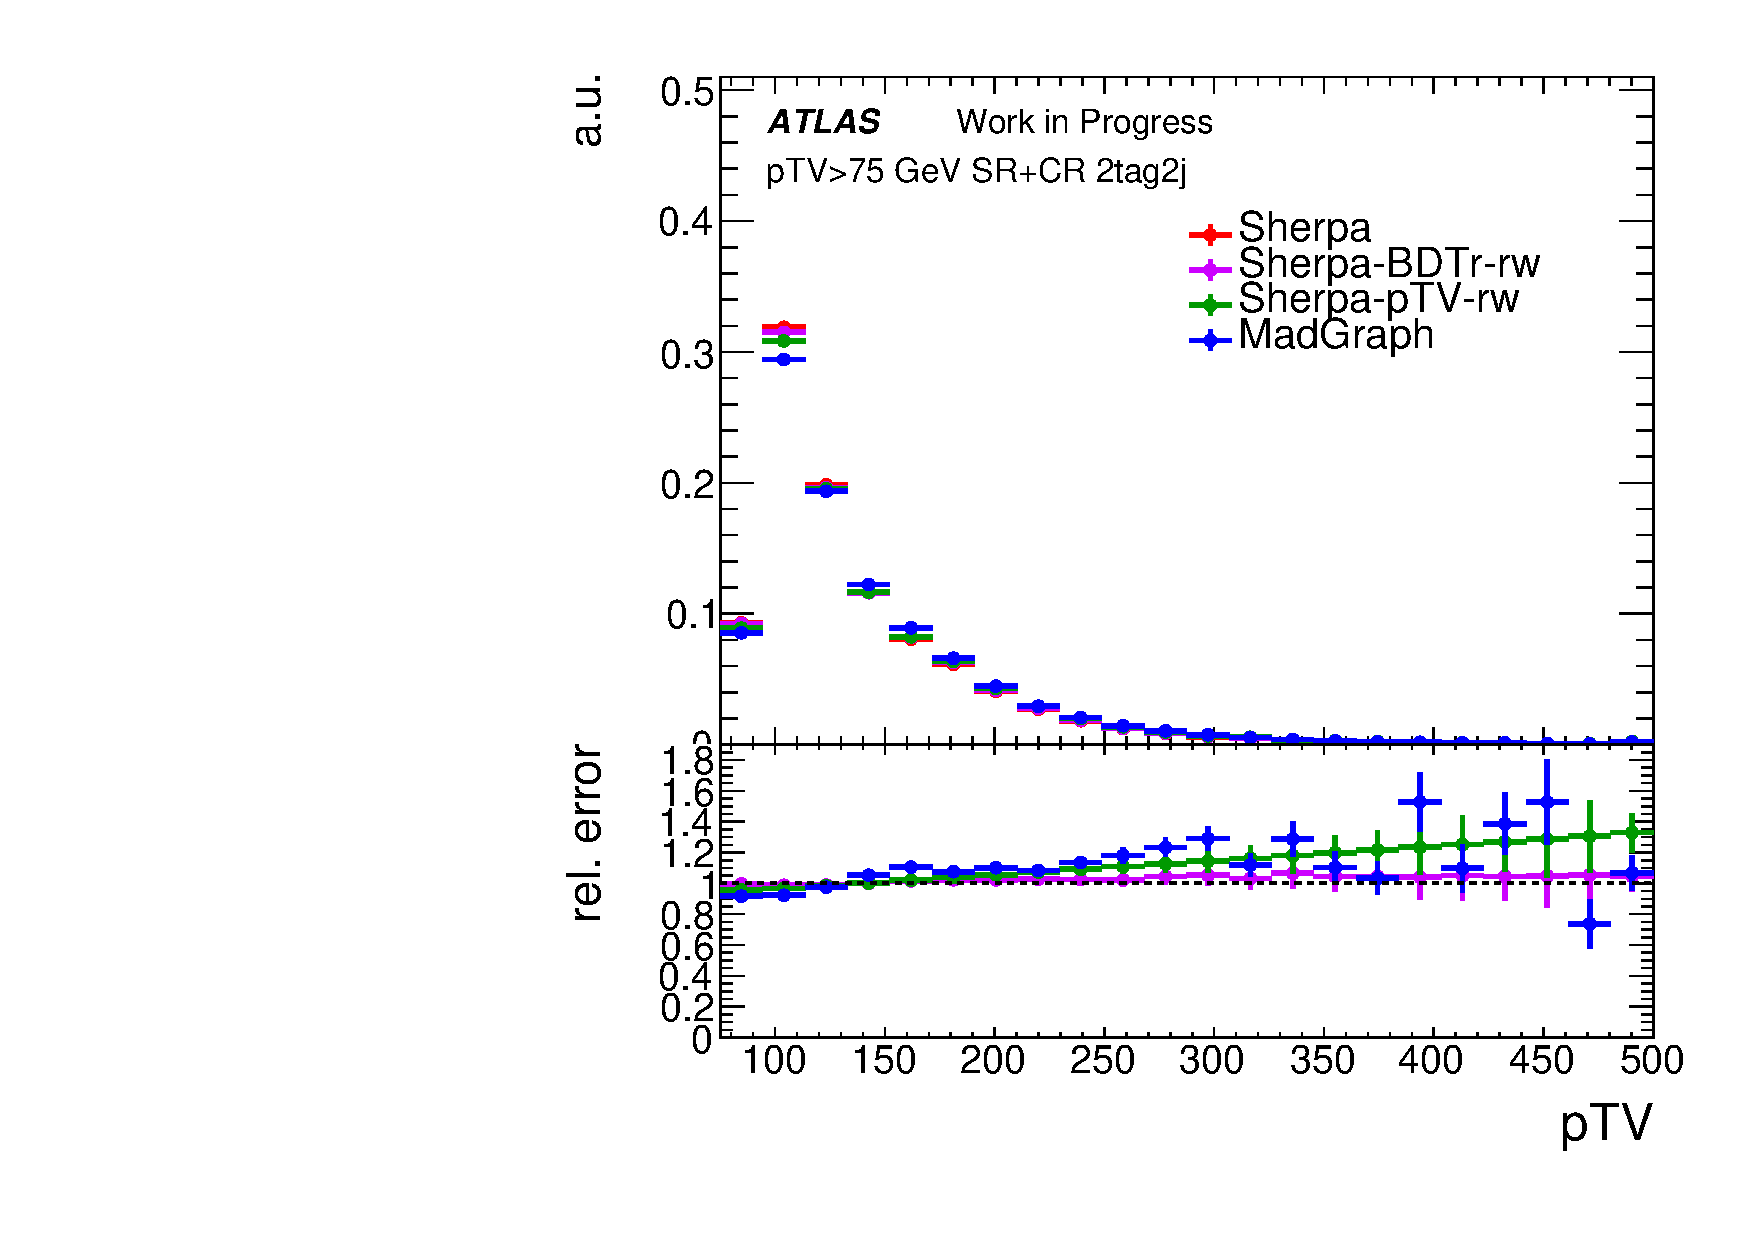
\includegraphics[width=0.45\textwidth]{figures/modelling_vjets/BDTreweighting/1Lep_pTVreweighting_shapes/1lepton_2tag2jet_75ptv_SR+CR_pTV_bb.pdf}}
%   \subfigure[$p_T^V$ 2tag 2jet
%   bc]{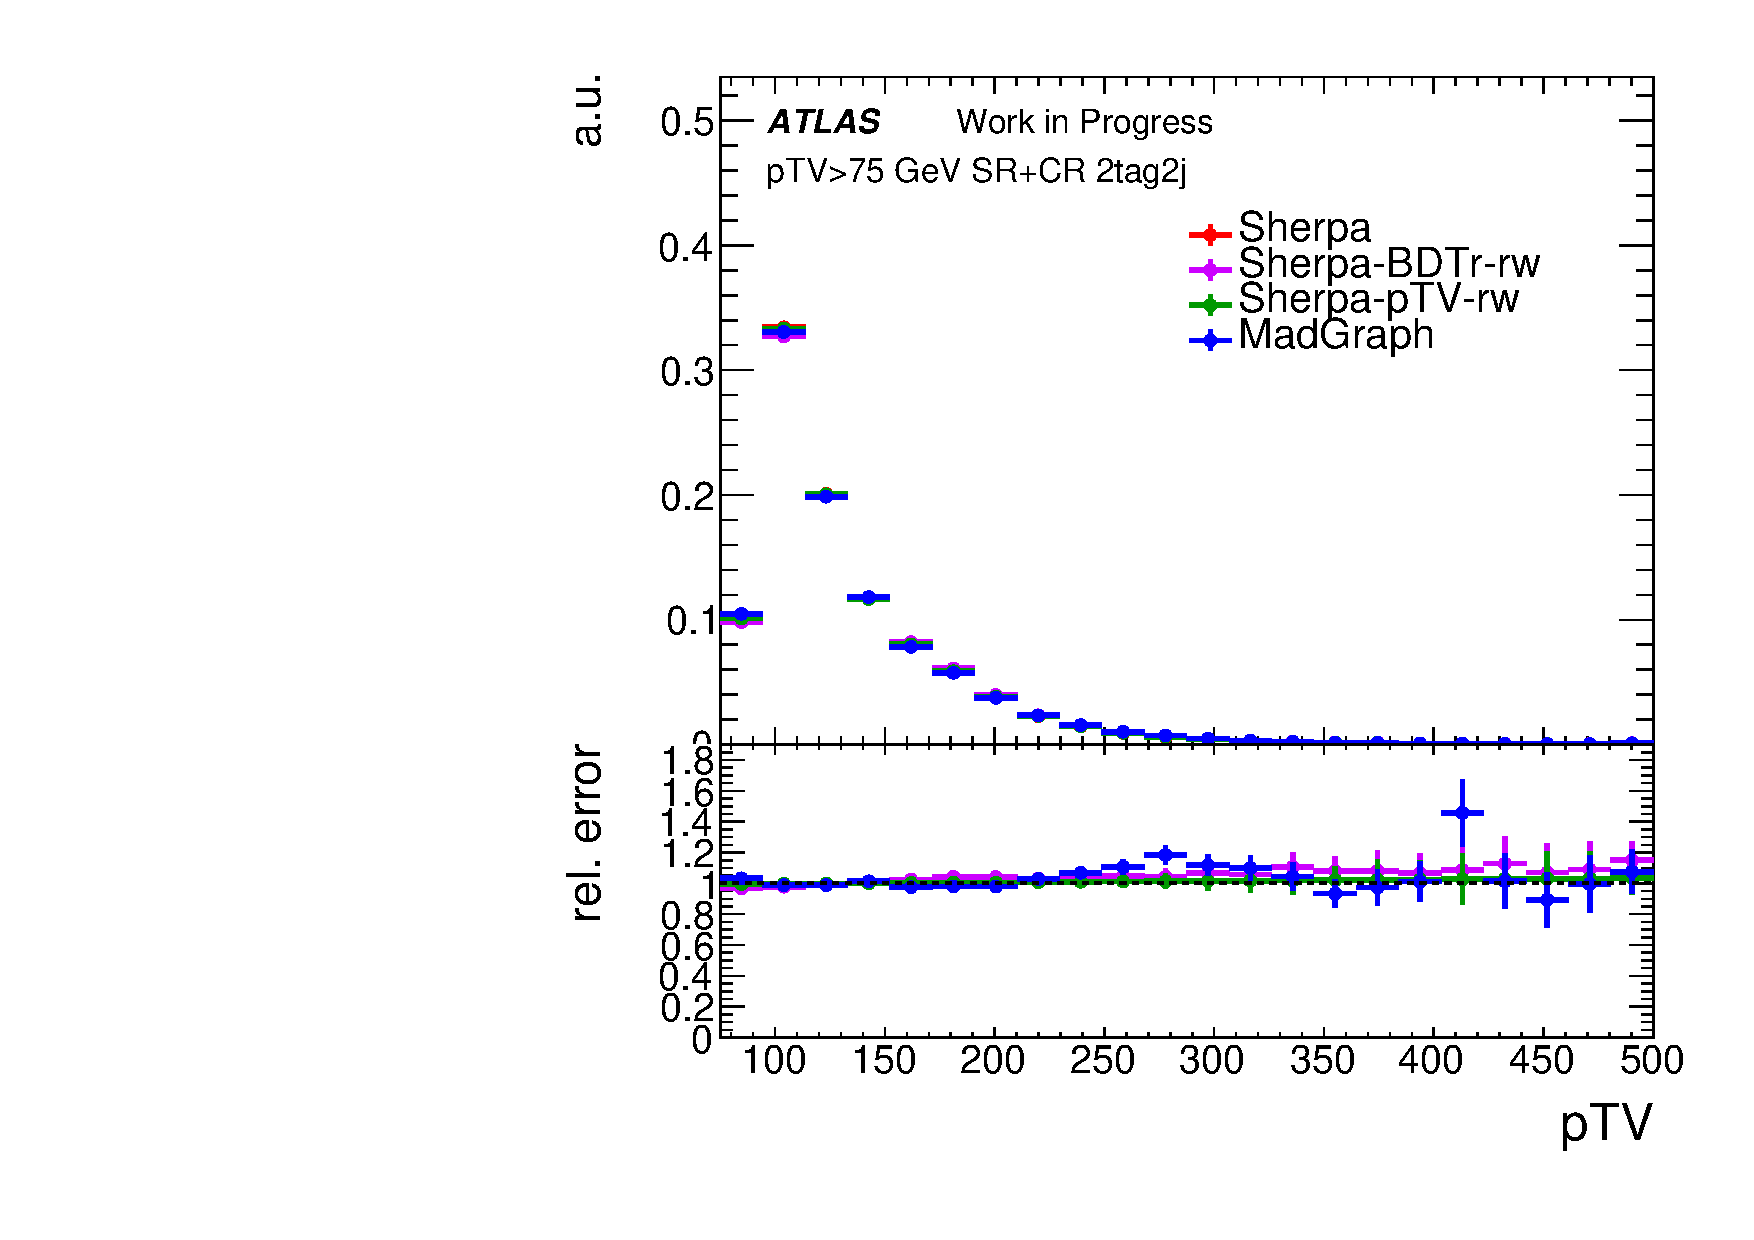
\includegraphics[width=0.45\textwidth]{figures/modelling_vjets/BDTreweighting/1Lep_pTVreweighting_shapes/1lepton_2tag2jet_75ptv_SR+CR_pTV_bc.pdf}}
% \\
% \subfigure[$p_T^V$ 2tag 2jet
% bl]{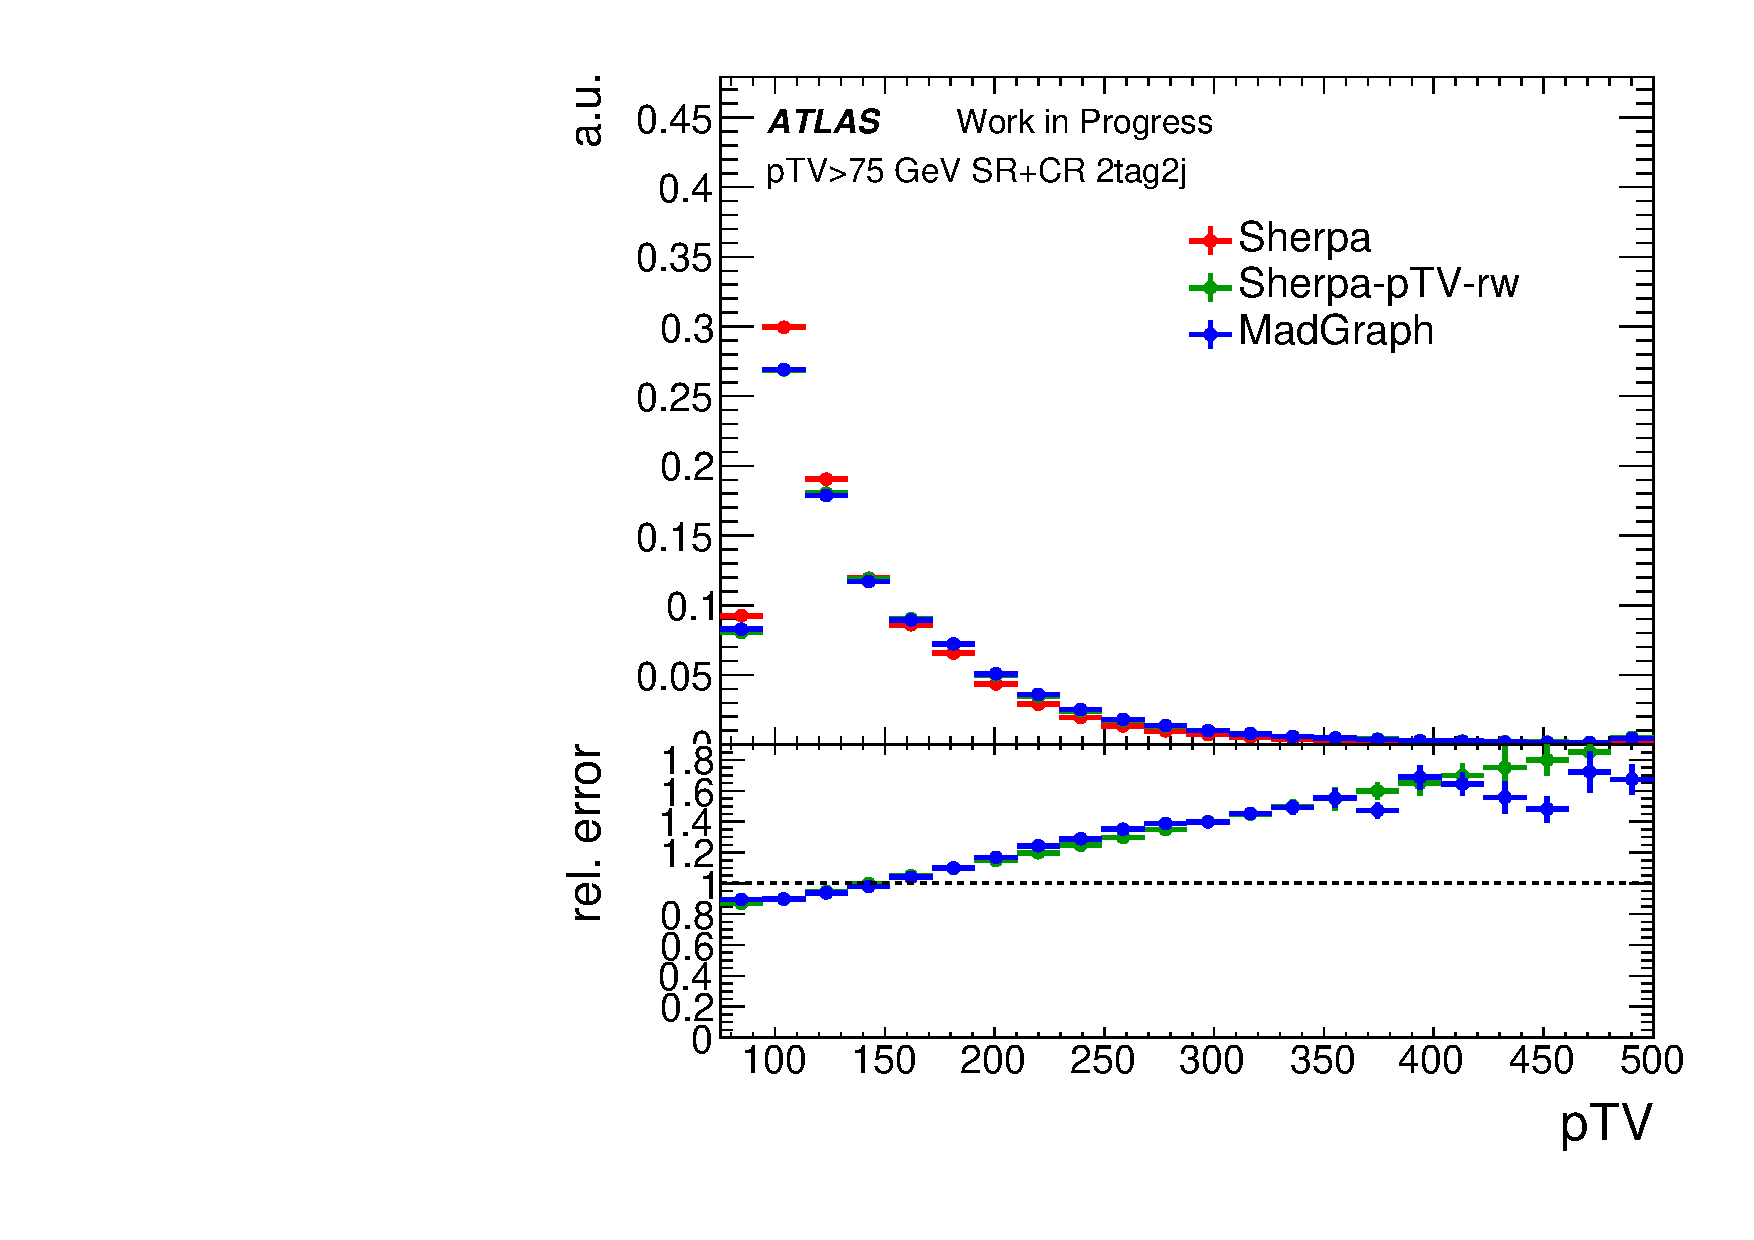
\includegraphics[width=0.45\textwidth]{figures/modelling_vjets/BDTreweighting/1Lep_pTVreweighting_shapes/1lepton_2tag2jet_75ptv_SR+CR_pTV_bl.pdf}}
% \subfigure[$p_T^V$ 2tag 2jet
% cc]{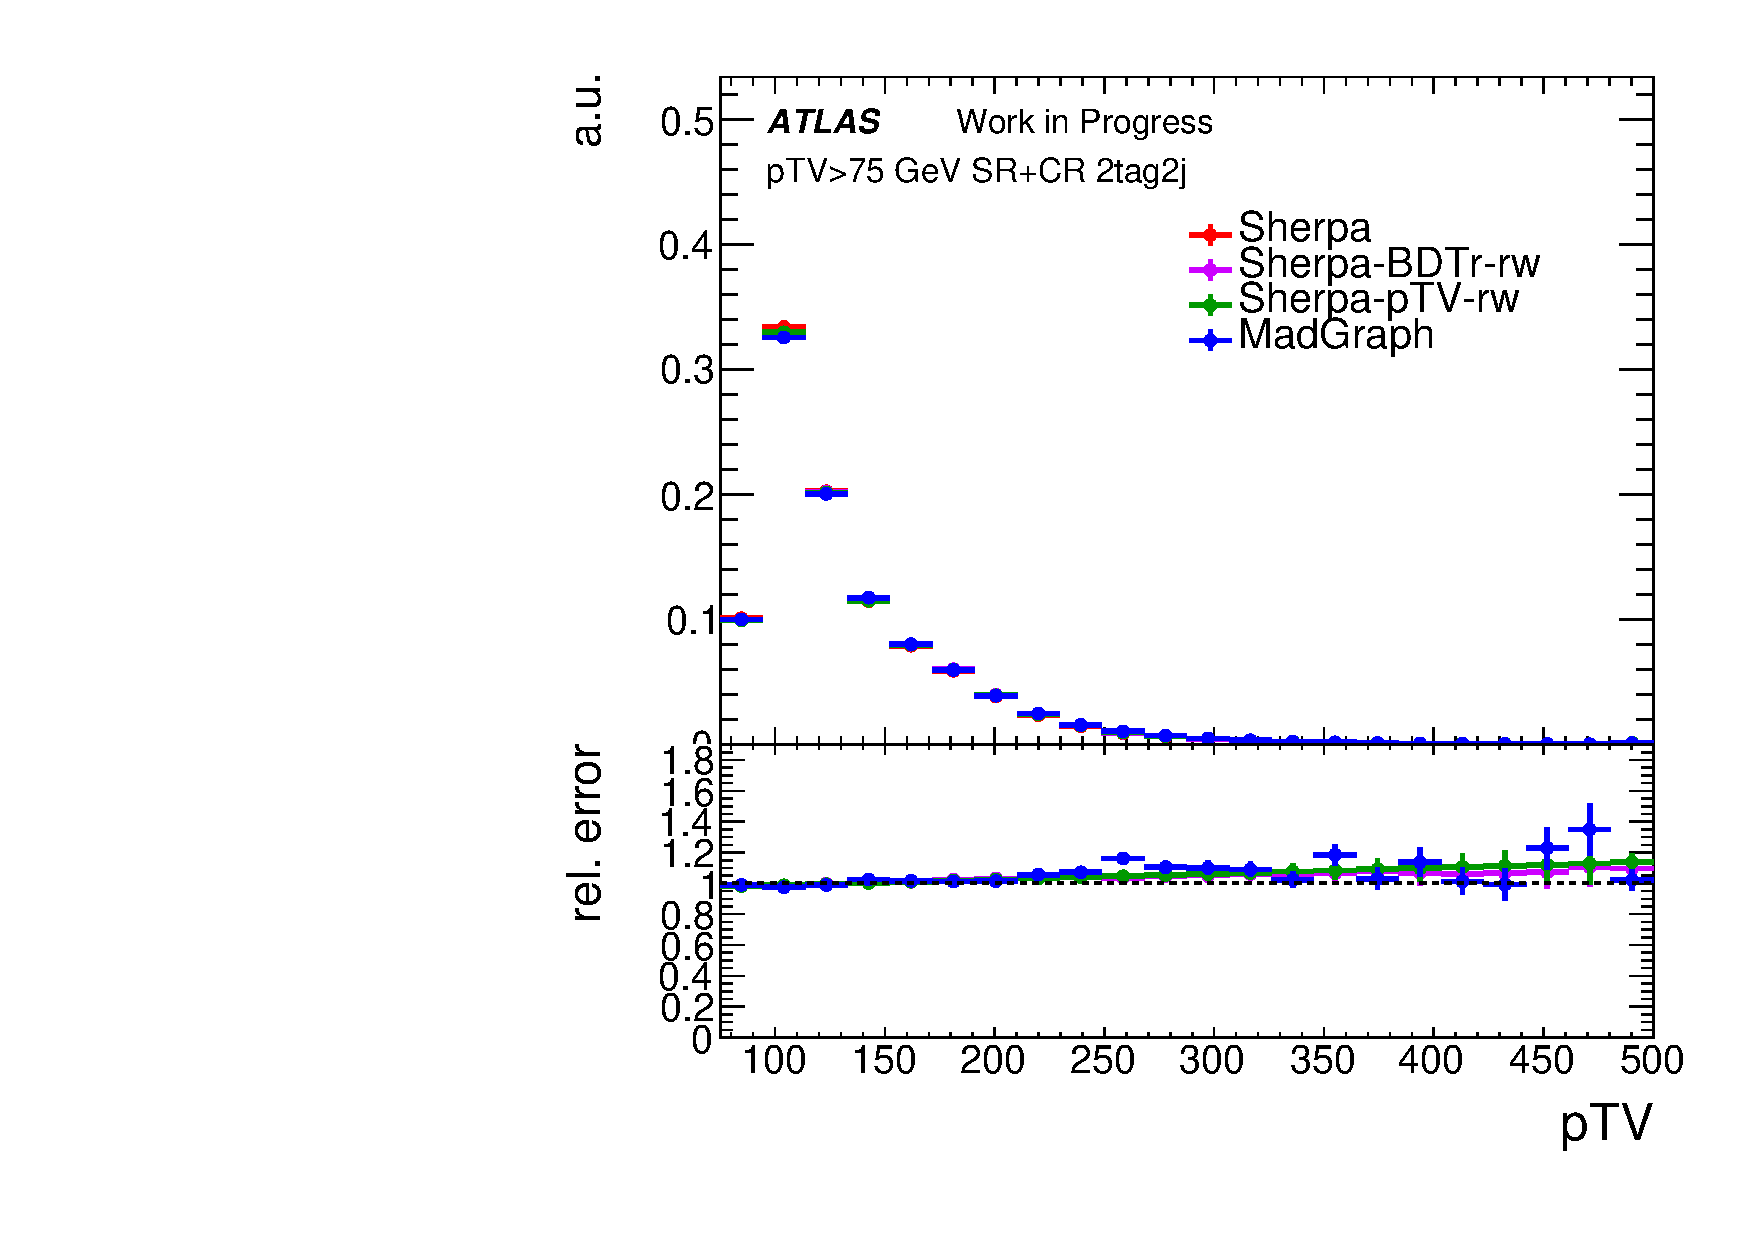
\includegraphics[width=0.45\textwidth]{figures/modelling_vjets/BDTreweighting/1Lep_pTVreweighting_shapes/1lepton_2tag2jet_75ptv_SR+CR_pTV_cc.pdf}}
% \\
% \caption{$p_T^V$ shape systematic in the 1-lepton channel for each heavy flavour
%   category and for the 2-jet category. The red and blue histograms correspond to
%   the $p_T^V$ distribution predicted by \textsc{Sherpa}~2.2.1 and \textsc{MadGraph}, respectively,
%   while the $p_T^V$ shape systematic is plotted in green.}
% \label{fig:wjets_1lep_2jet_SysWPtVBDTr}
% \end{center}
% \end{figure}

% \begin{figure}[H]
% \begin{center}
%   \subfigure[$p_T^V$ 2tag 3jet
%   bb]{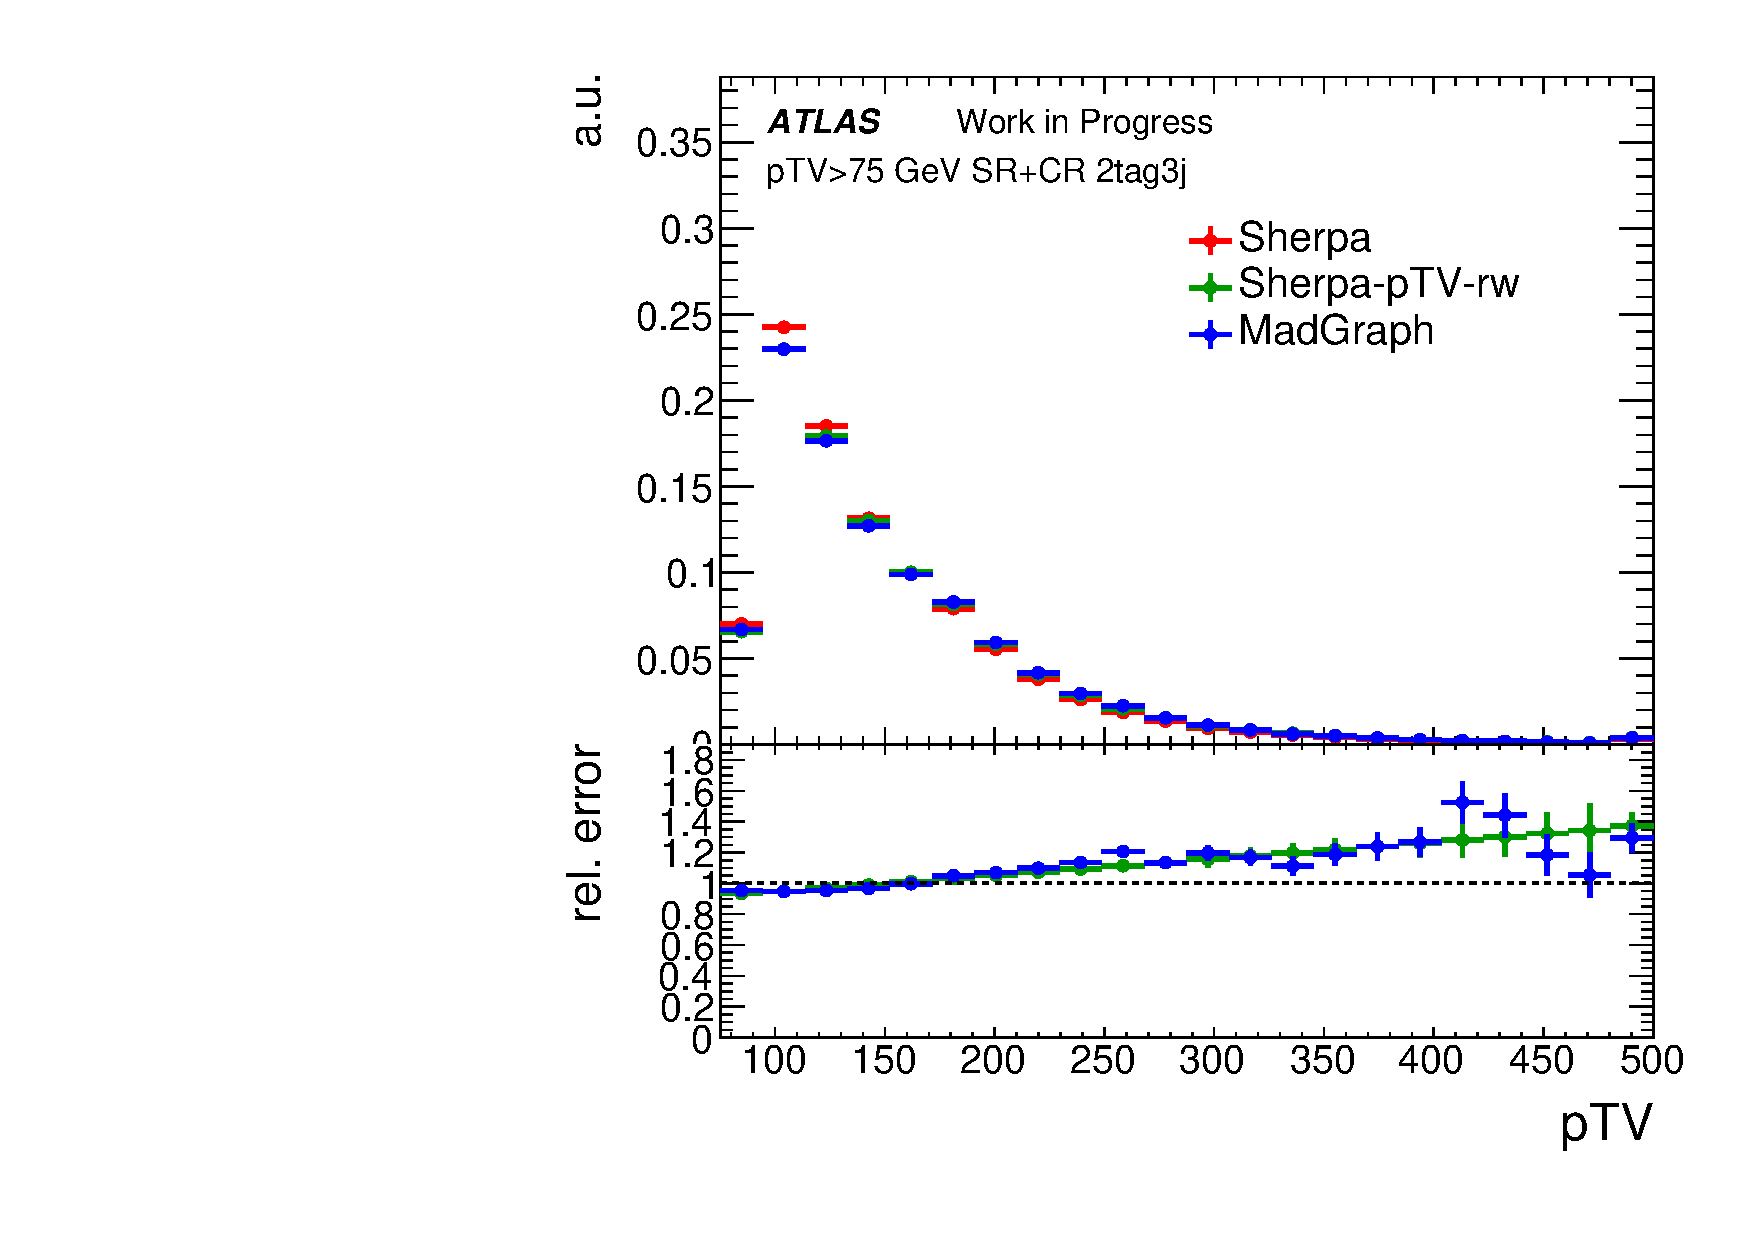
\includegraphics[width=0.45\textwidth]{figures/modelling_vjets/BDTreweighting/1Lep_pTVreweighting_shapes/1lepton_2tag3jet_75ptv_SR+CR_pTV_bb.pdf}}
%   \subfigure[$p_T^V$ 2tag 3jet
%   bc]{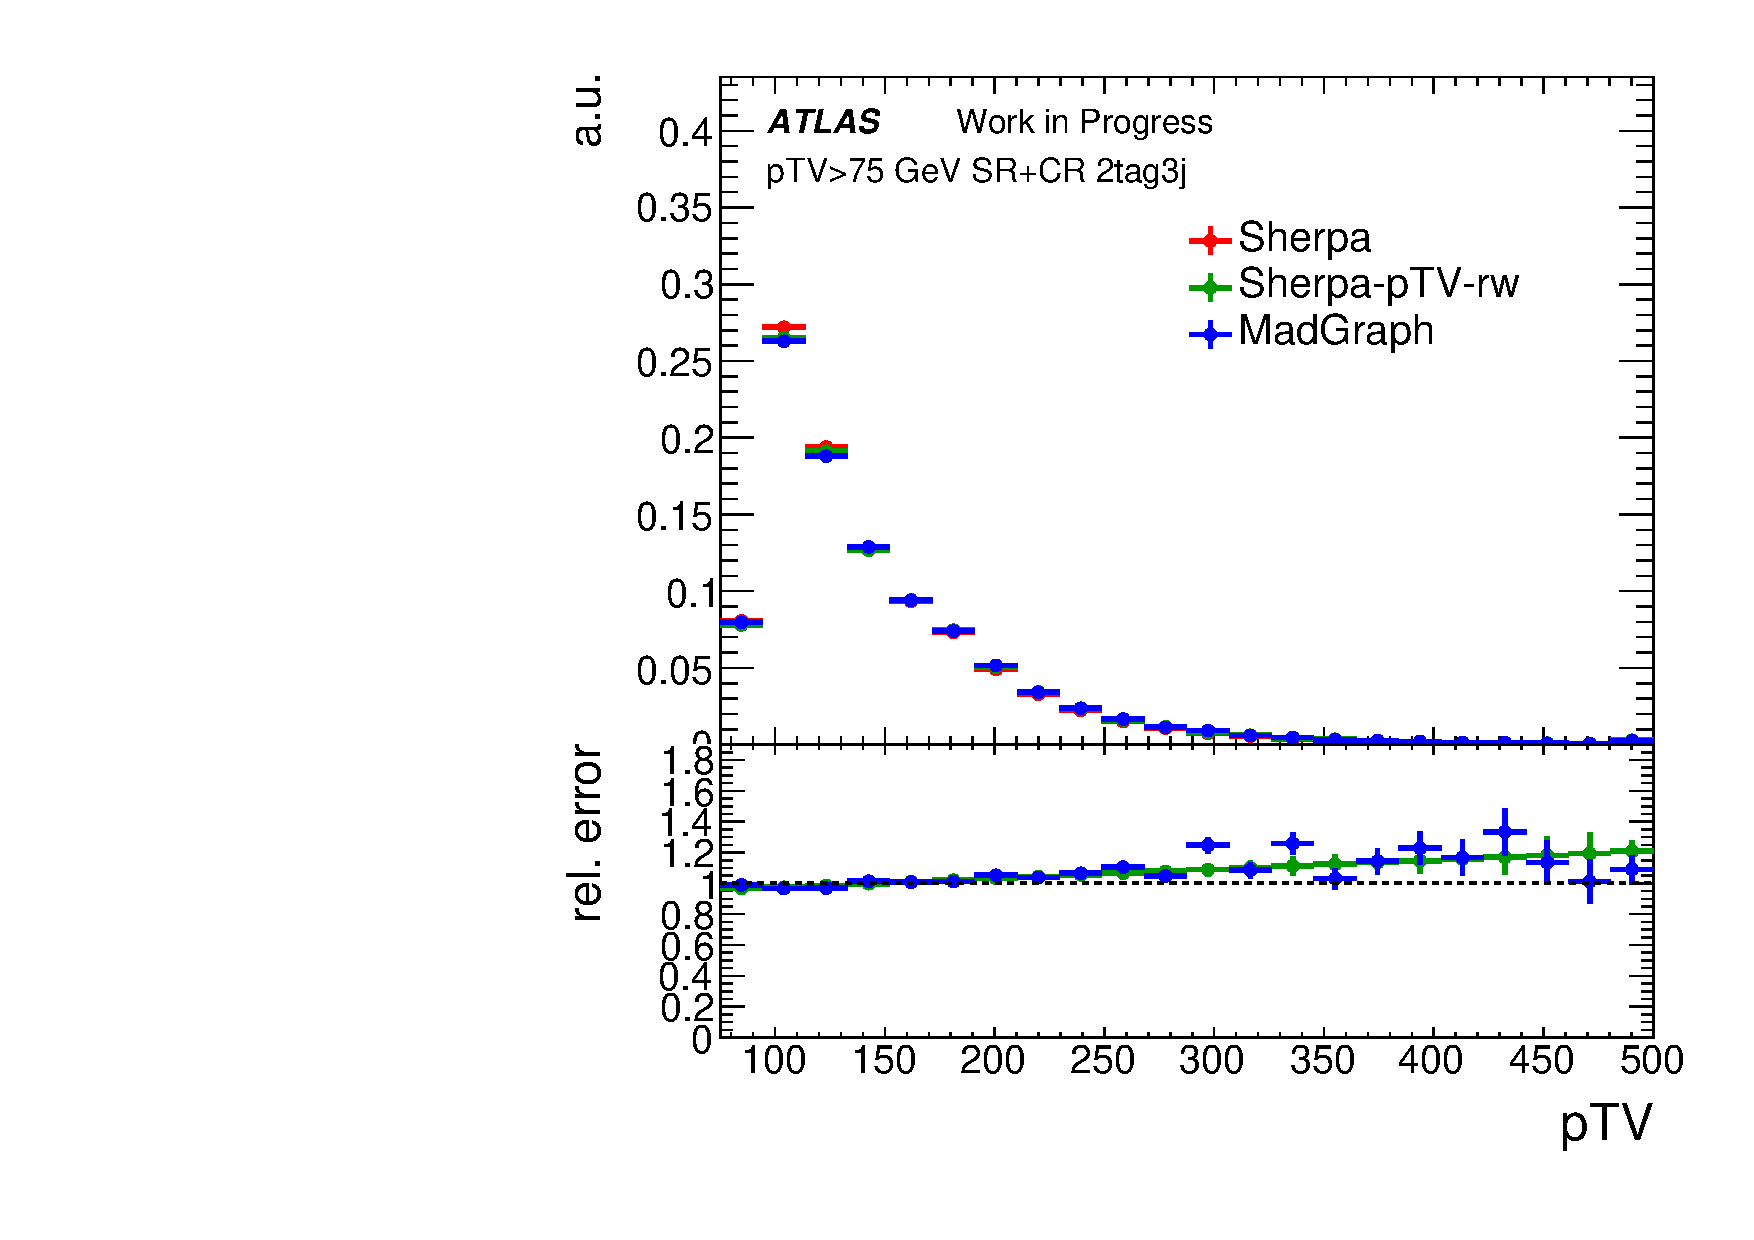
\includegraphics[width=0.45\textwidth]{figures/modelling_vjets/BDTreweighting/1Lep_pTVreweighting_shapes/1lepton_2tag3jet_75ptv_SR+CR_pTV_bc.pdf}}
%   \\
%   \subfigure[$p_T^V$ 2tag 3jet
%   bl]{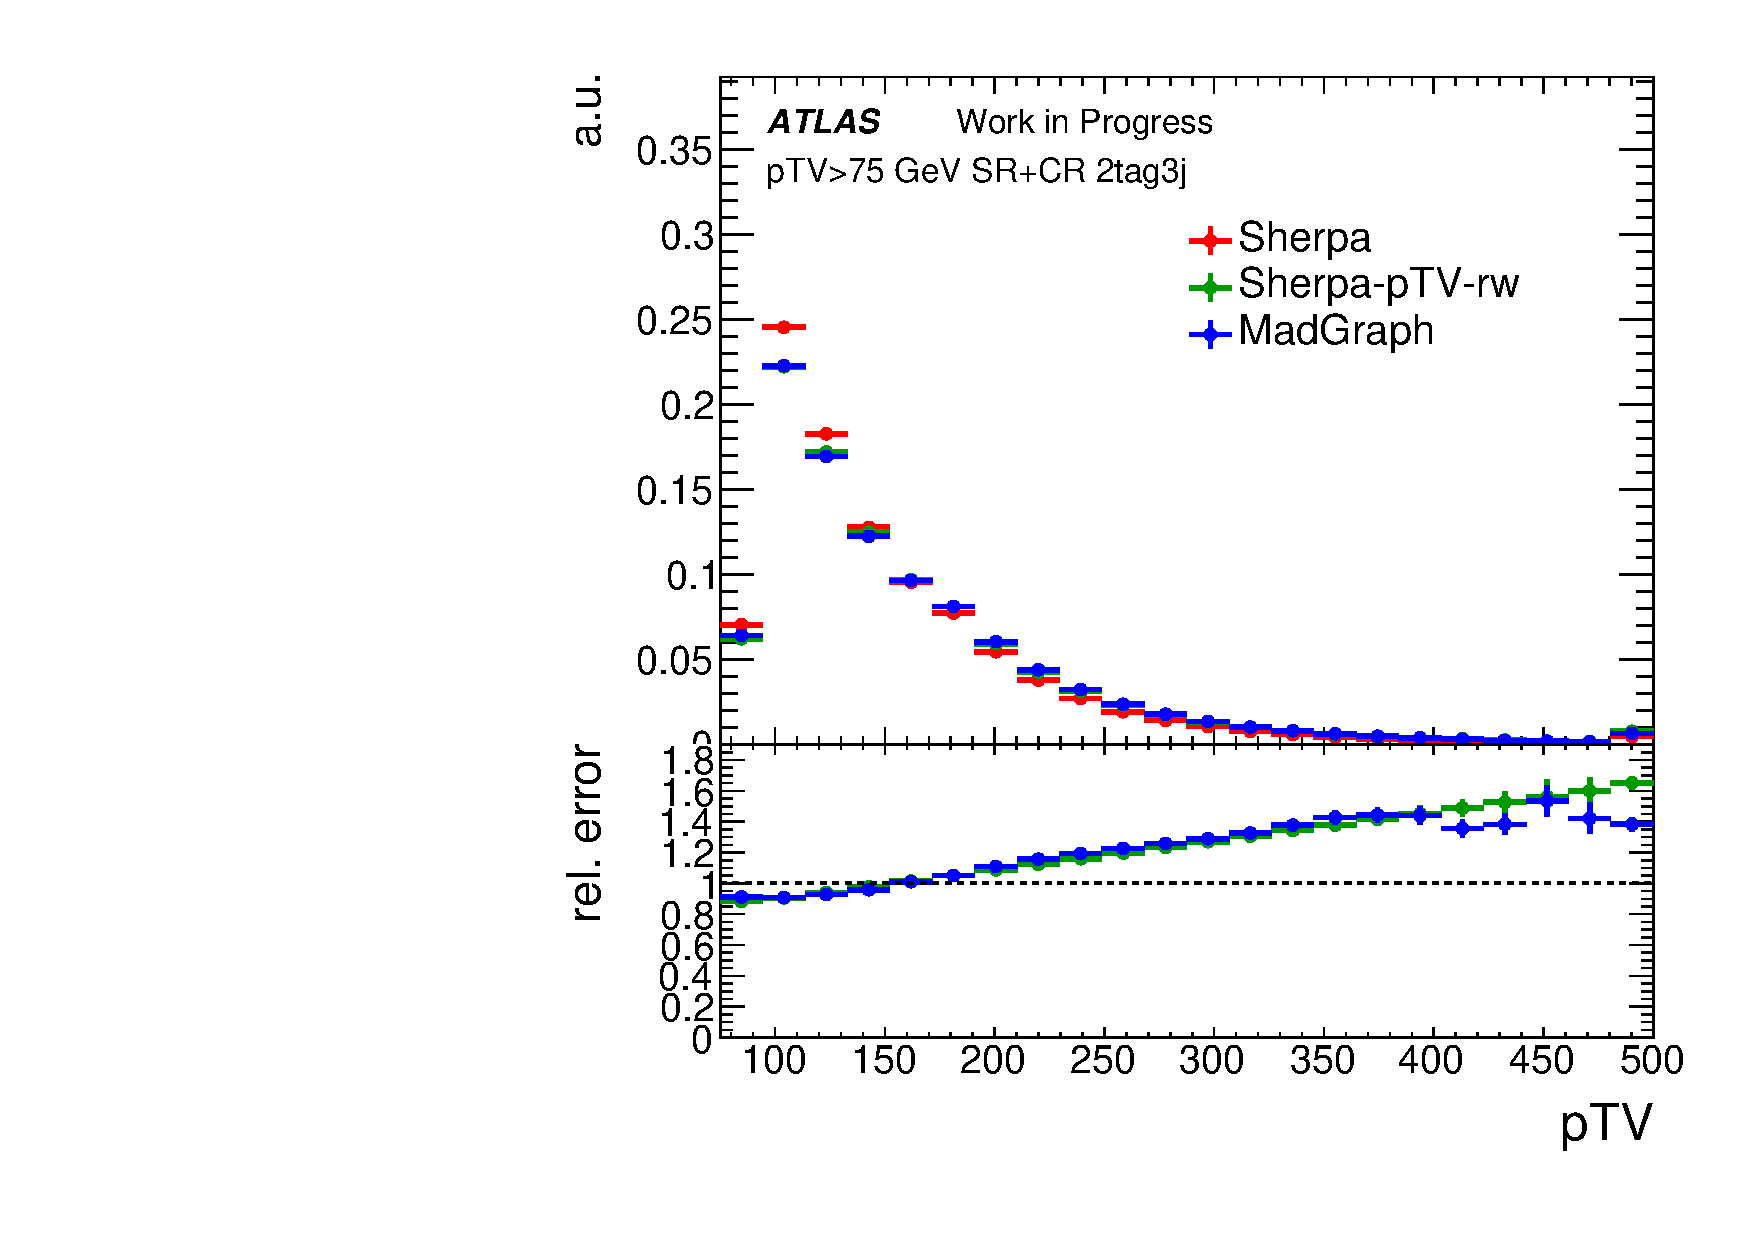
\includegraphics[width=0.45\textwidth]{figures/modelling_vjets/BDTreweighting/1Lep_pTVreweighting_shapes/1lepton_2tag3jet_75ptv_SR+CR_pTV_bl.pdf}}
%   \subfigure[$p_T^V$ 2tag 3jet
%   cc]{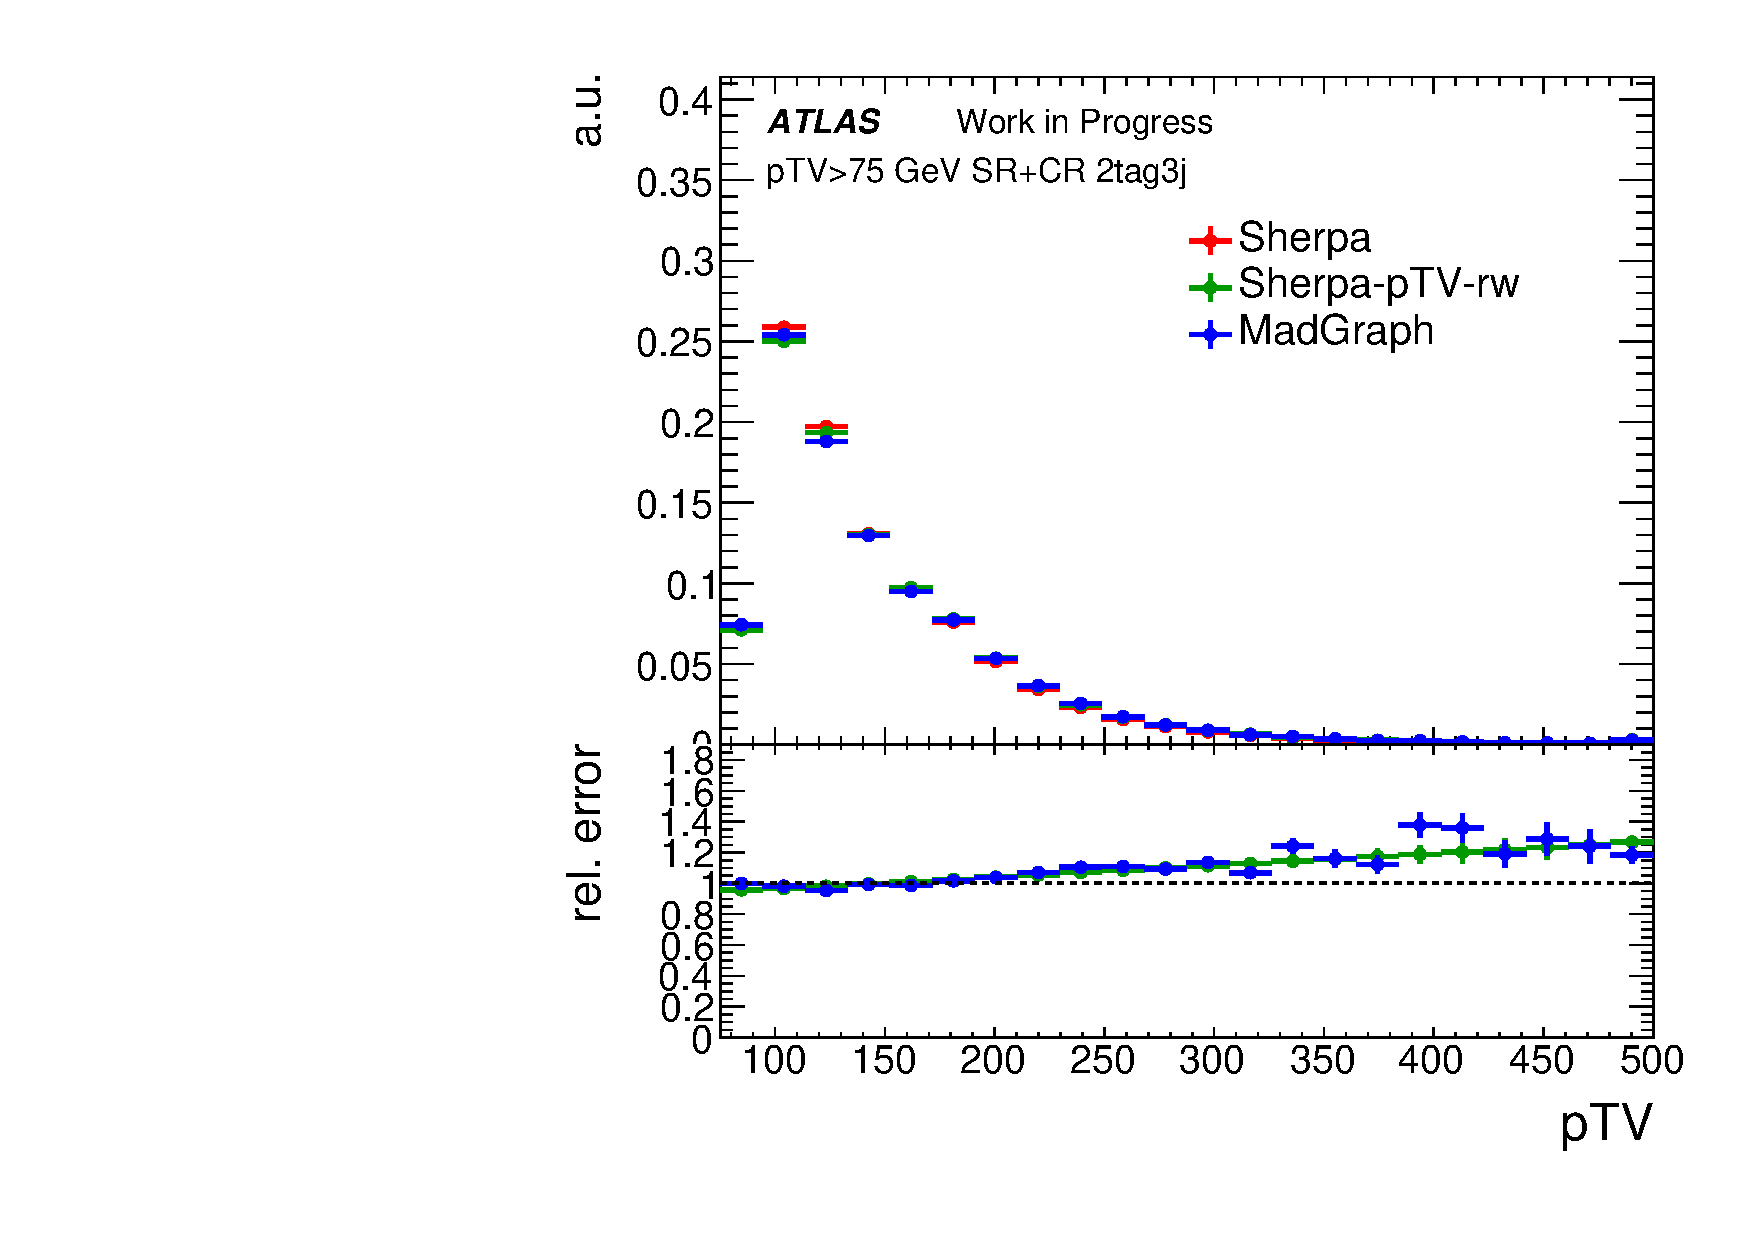
\includegraphics[width=0.45\textwidth]{figures/modelling_vjets/BDTreweighting/1Lep_pTVreweighting_shapes/1lepton_2tag3jet_75ptv_SR+CR_pTV_cc.pdf}}
%   \\
% \caption{$p_T^V$ shape systematic in the 1-lepton channel for each heavy flavour
%   category and for the 3-jet category. The red and blue histograms correspond to
%   the $p_T^V$ distribution predicted by \textsc{Sherpa}~2.2.1 and
%   \textsc{MadGraph}, respectively, while the $p_T^V$ shape systematic is plotted
%   in green.}
% \label{fig:wjets_1lep_3jet_SysWPtVBDTr}
% \end{center}
% \end{figure}

% Given the low statistics in the 0-lepton channel, the $p_T^V$ shapes derived in
% the 1-lepton channel are also used in the 0-lepton channel. The goodness of this
% approach is showed in Figure~\ref{fig:wjets_01lep_2jet_SysWPtVBDTr} for the
% 2tag2jet category and in Figure~\ref{fig:wjets_01lep_3jet_SysWPtVBDTr} for the
% 2tag3jet region for each heavy flavour pair. An offset between the $p_T^V$ and the
% MET shapes in the two channels can be seen, especially in the $W$+bl events.
% This is due to the fact that the $p_T^V$ shape is derived from a unit-normalized
% ratio between \textsc{Sherpa}~2.2.1 and \textsc{MadGraph} in the $p_T^V > 75$ \GeV  range, while
% the MET distribution is normalized to 1 in the MET $>150$ \GeV range. This is
% confirmed by the example plot in
% Figure~\ref{fig:wjets_01lep_2jet_bl_SysWPtVBDTr_From150} where both the $p_T^V$
% and the MET shape in the 2tag2jet region have been normalized to 1 in the
% $p_T^V$(MET) $>150$ \GeV range.

% \begin{figure}[H]
% \begin{center}
% \subfigure[2tag 2jet
% bb]{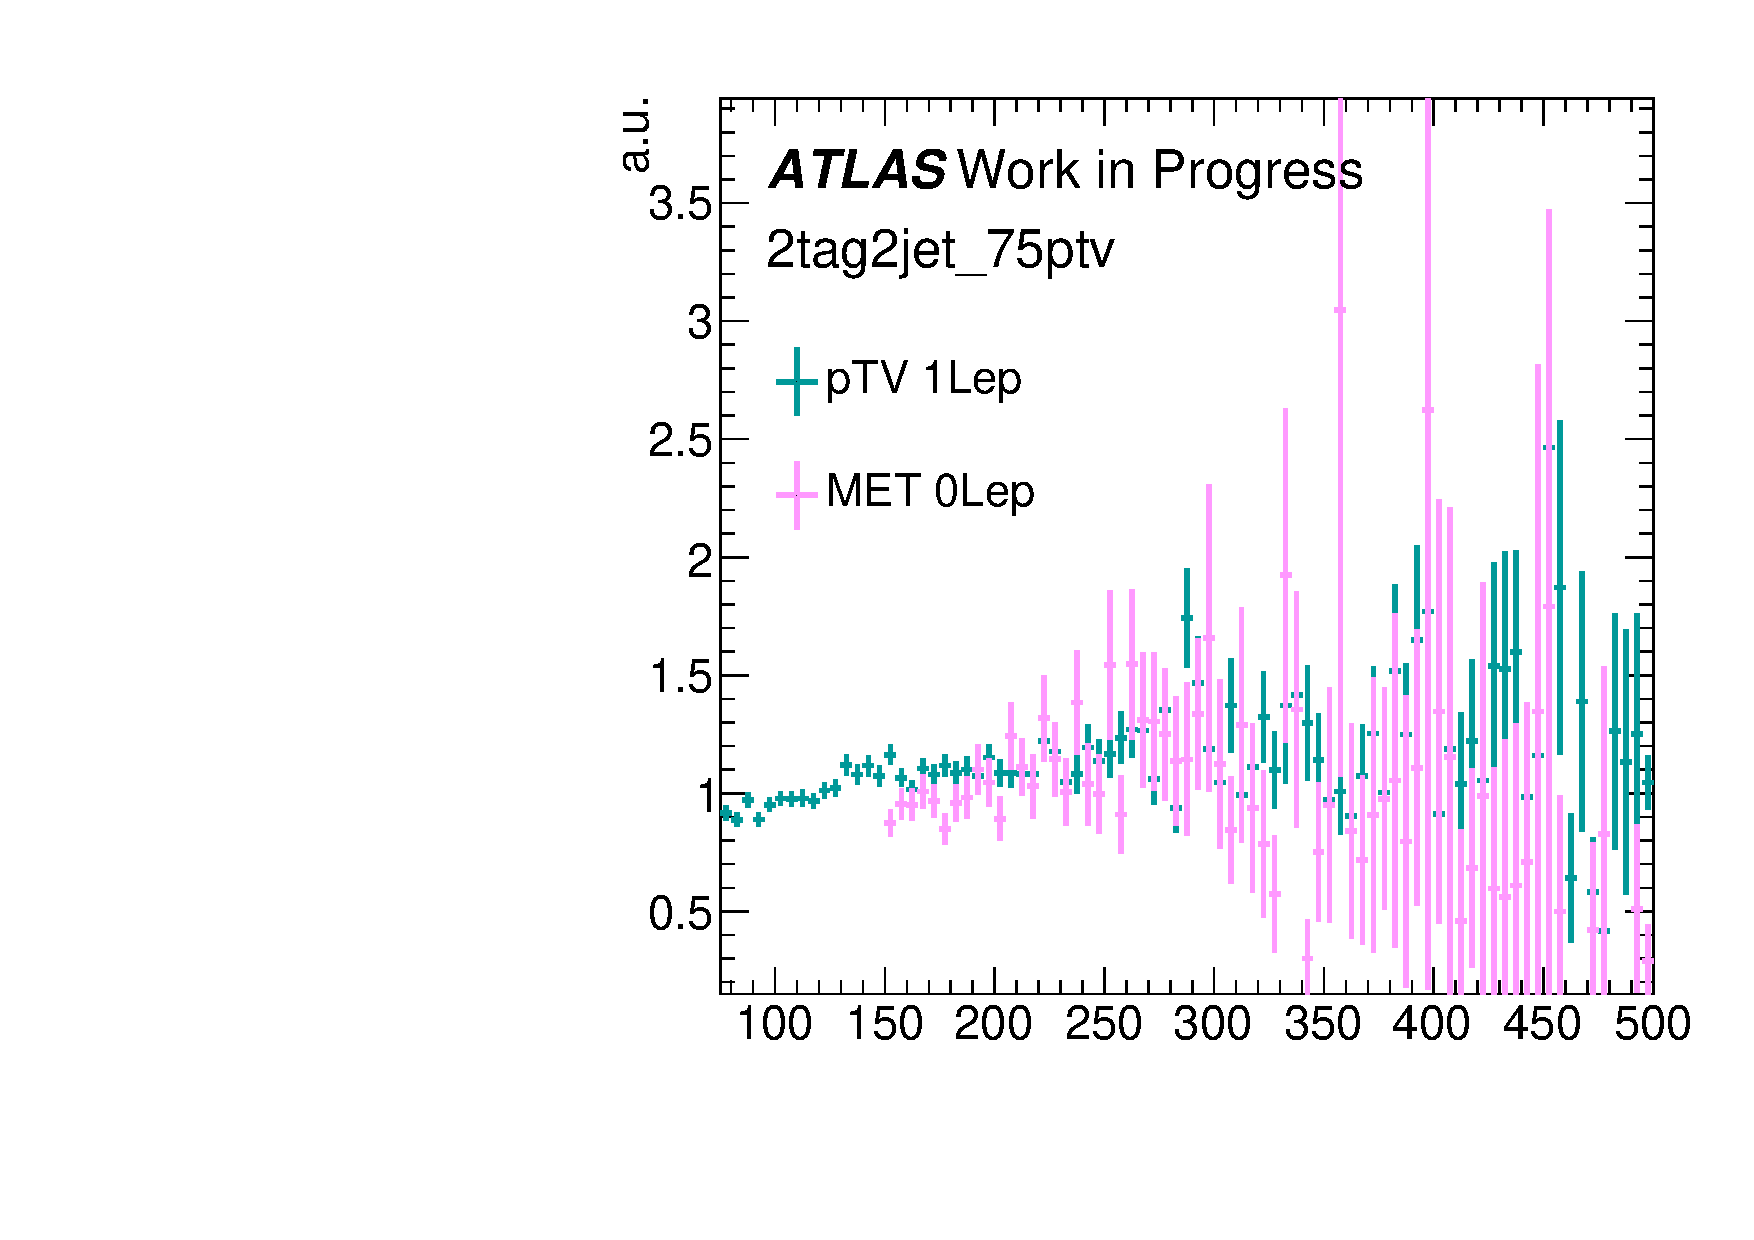
\includegraphics[width=0.45\textwidth]{figures/modelling_vjets/BDTreweighting/01Lep_reweighting_shapes/ReweightingVarComparison_2tag2jet_75ptv_bb.pdf}}
% \subfigure[2tag 2jet
% bc]{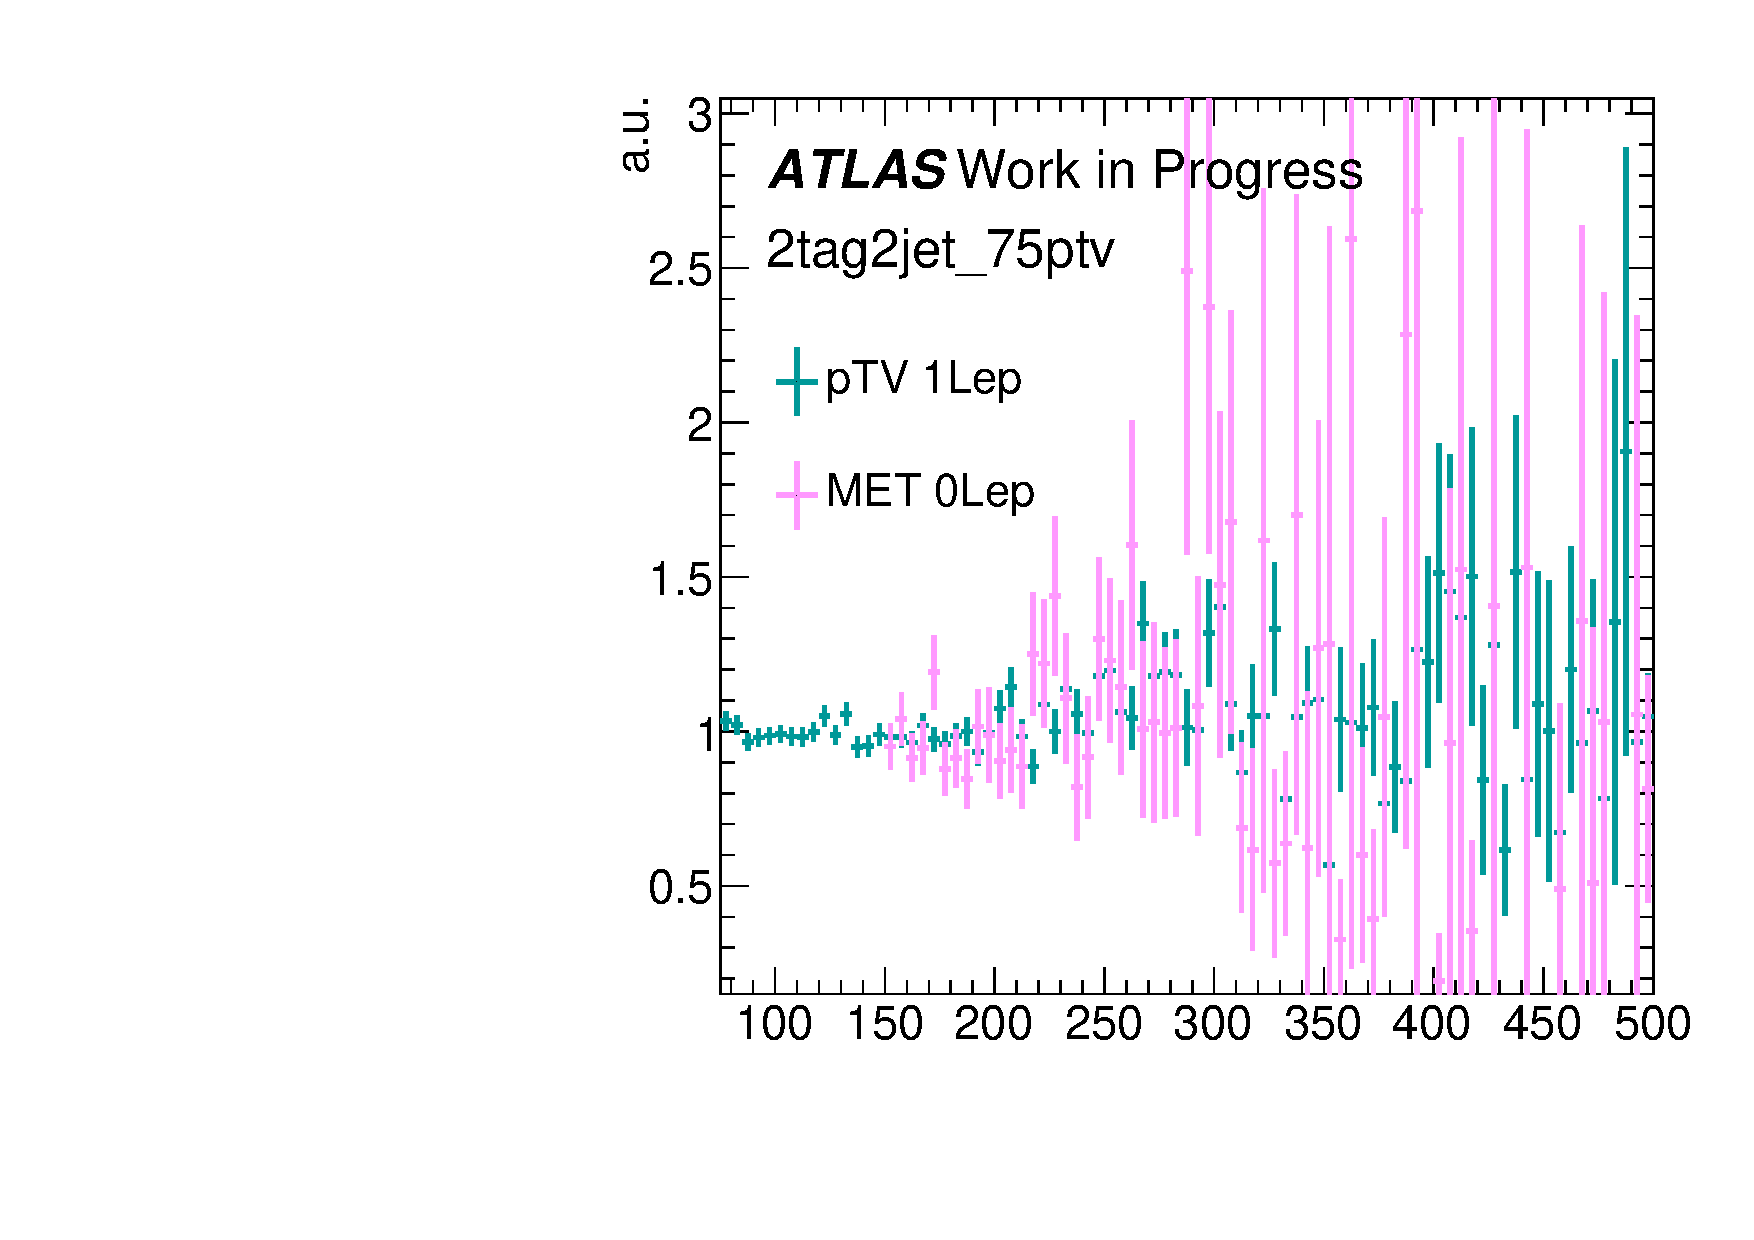
\includegraphics[width=0.45\textwidth]{figures/modelling_vjets/BDTreweighting/01Lep_reweighting_shapes/ReweightingVarComparison_2tag2jet_75ptv_bc.pdf}}
% \\
% \subfigure[2tag 2jet
% bl]{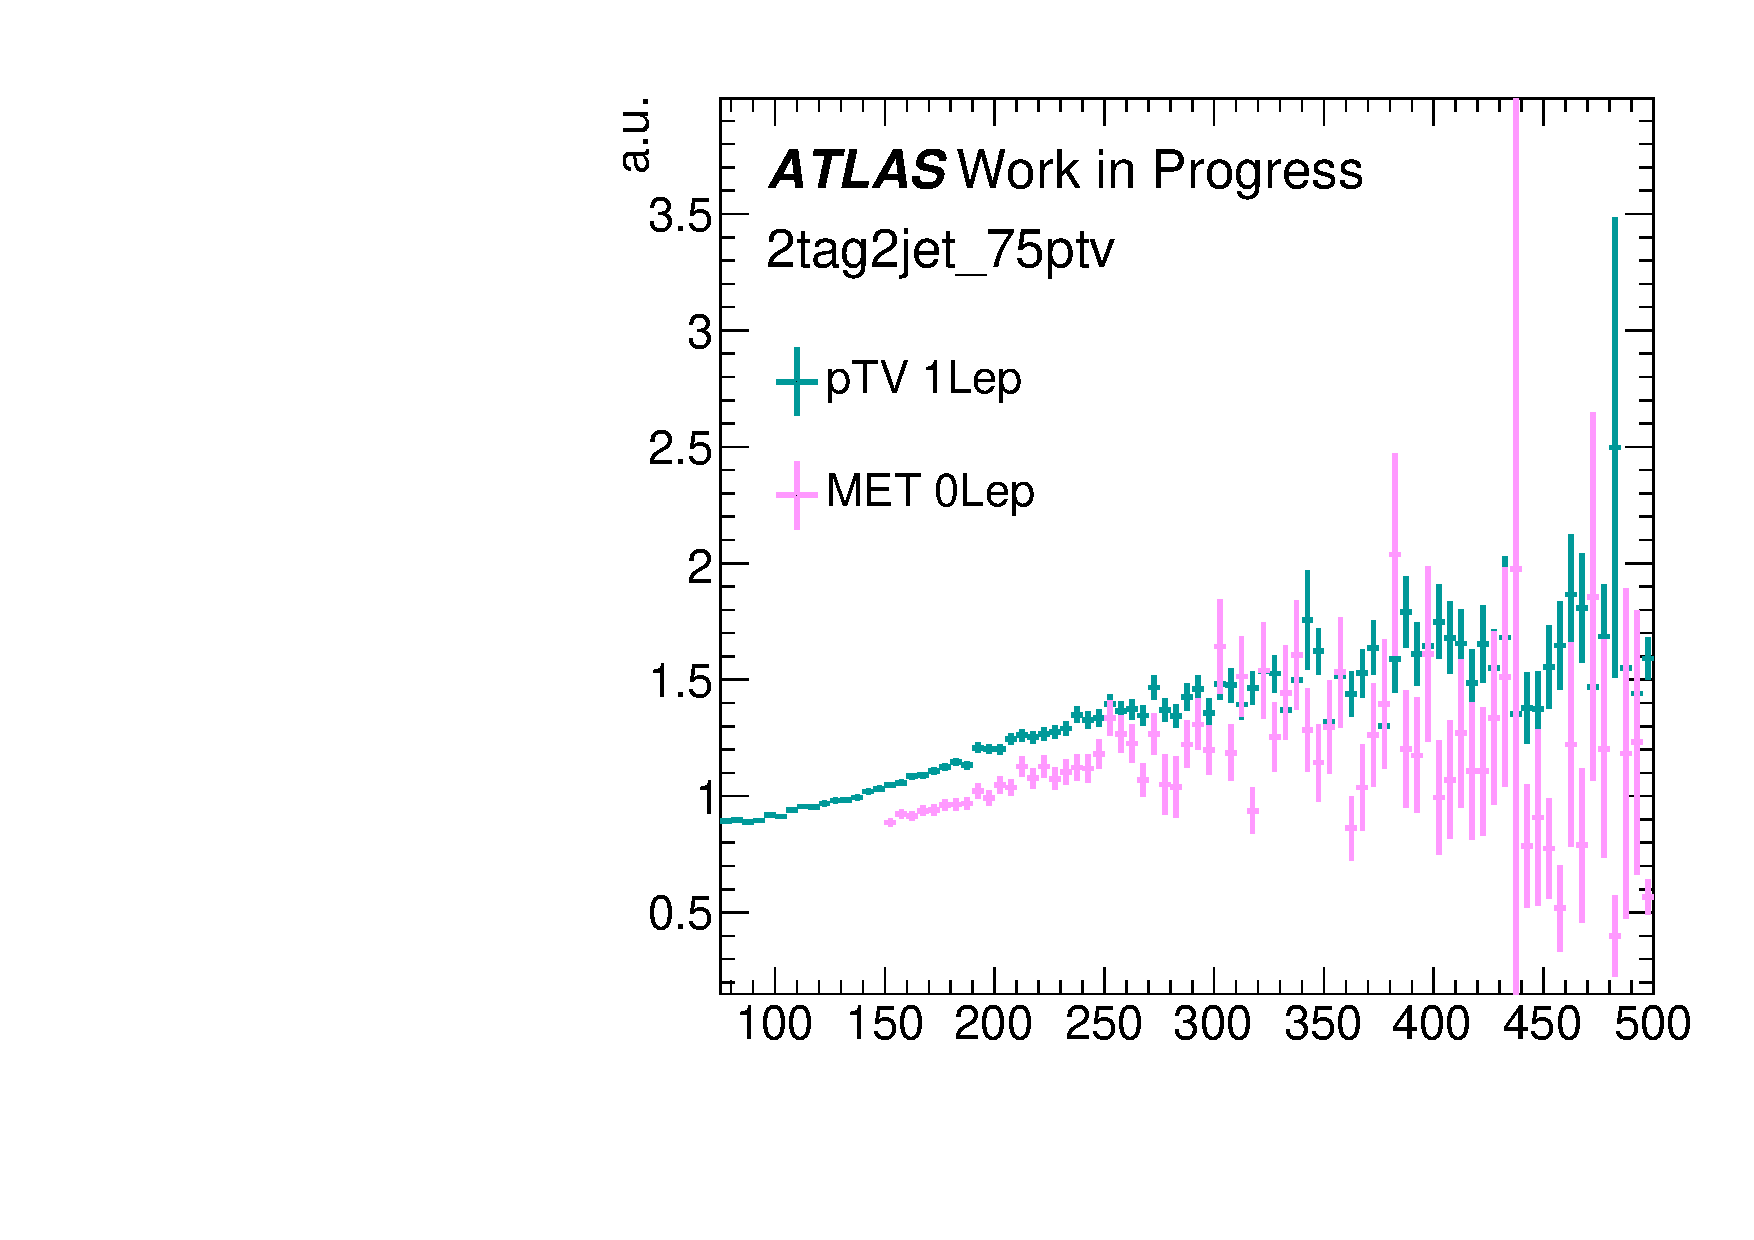
\includegraphics[width=0.45\textwidth]{figures/modelling_vjets/BDTreweighting/01Lep_reweighting_shapes/ReweightingVarComparison_2tag2jet_75ptv_bl.pdf}}
% \subfigure[2tag 2jet
% cc]{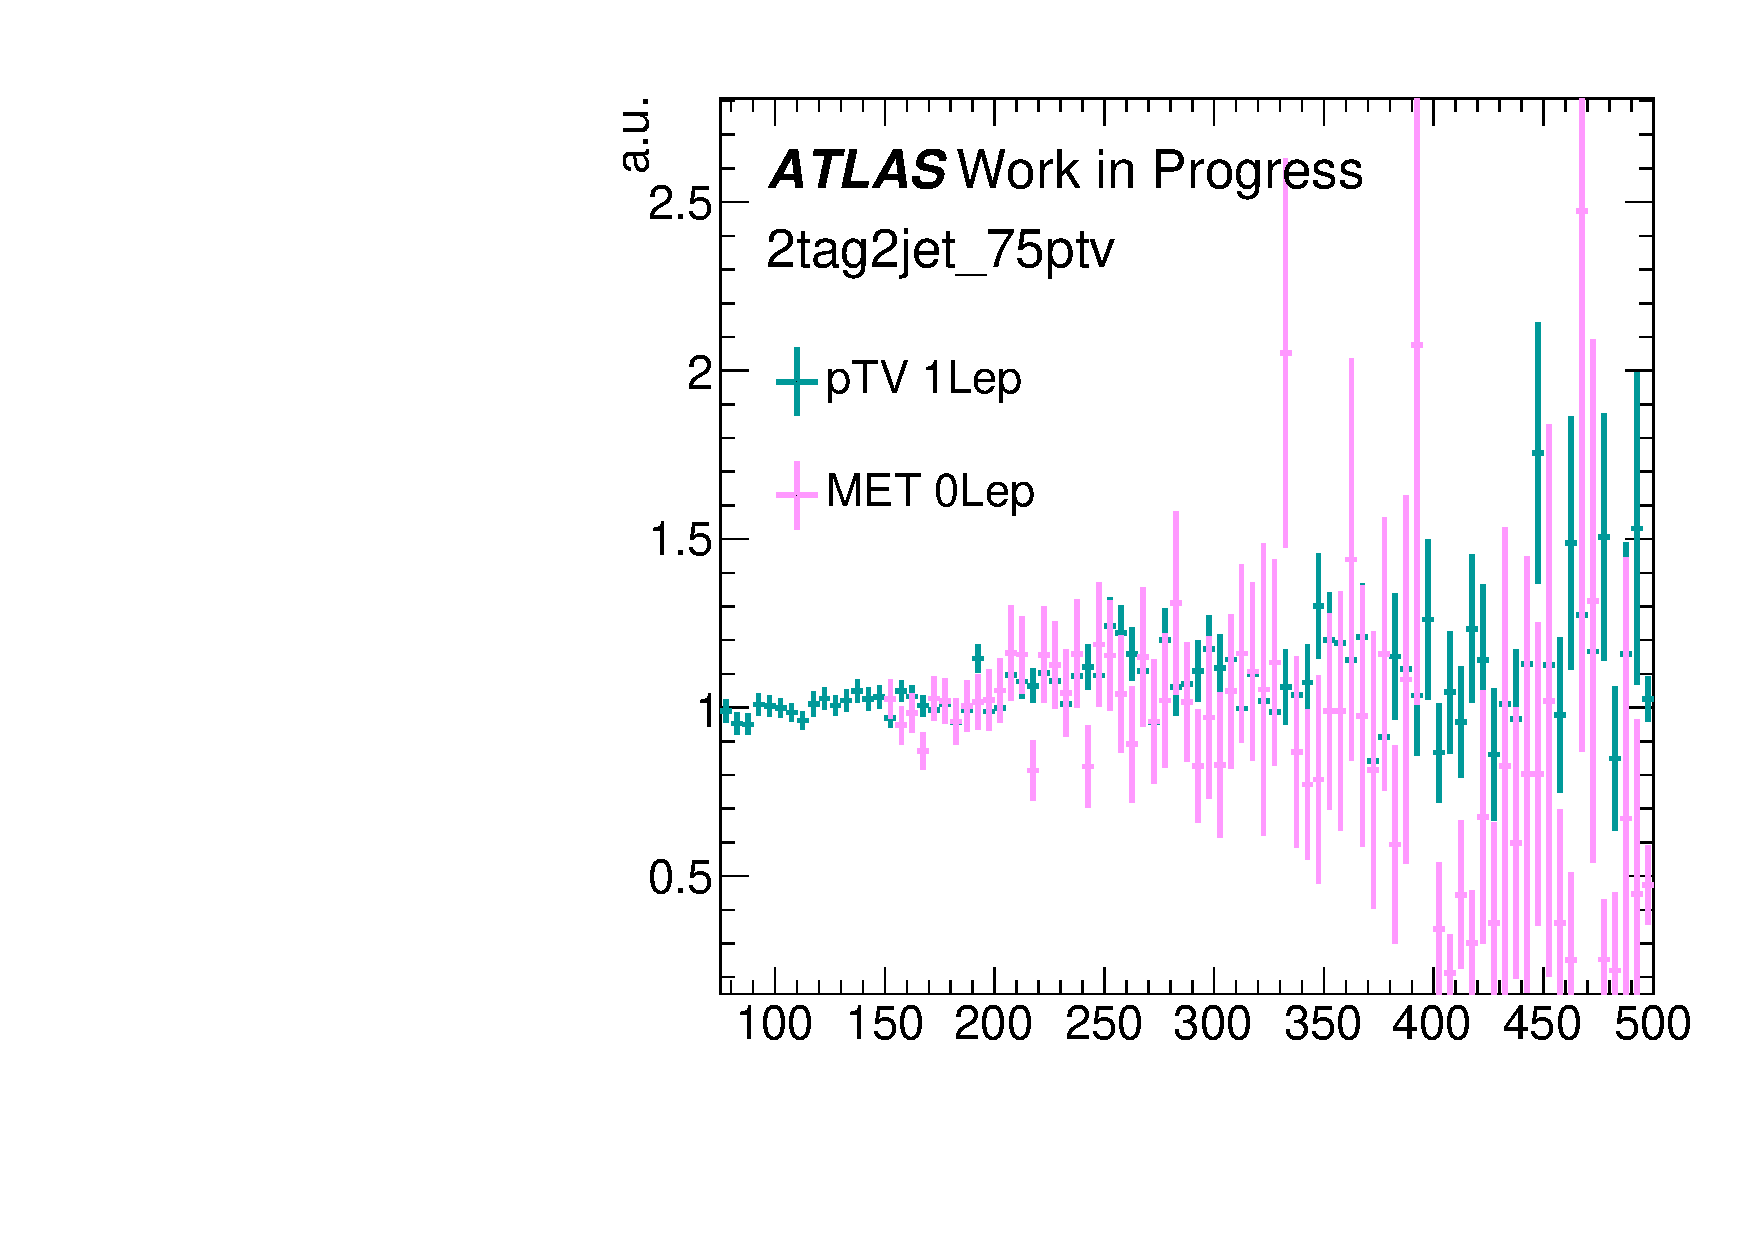
\includegraphics[width=0.45\textwidth]{figures/modelling_vjets/BDTreweighting/01Lep_reweighting_shapes/ReweightingVarComparison_2tag2jet_75ptv_cc.pdf}}
% \\
% \caption{$p_T^V$ and MET shape systematics derived in the 2tag2jet region of the
%   1-lepton and 0-lepton channels, respectively, for each heavy flavour pair.}
% \label{fig:wjets_01lep_2jet_SysWPtVBDTr}
% \end{center}
% \end{figure}

% \begin{figure}[H]
% \begin{center}
% \subfigure[2tag 3jet
% bb]{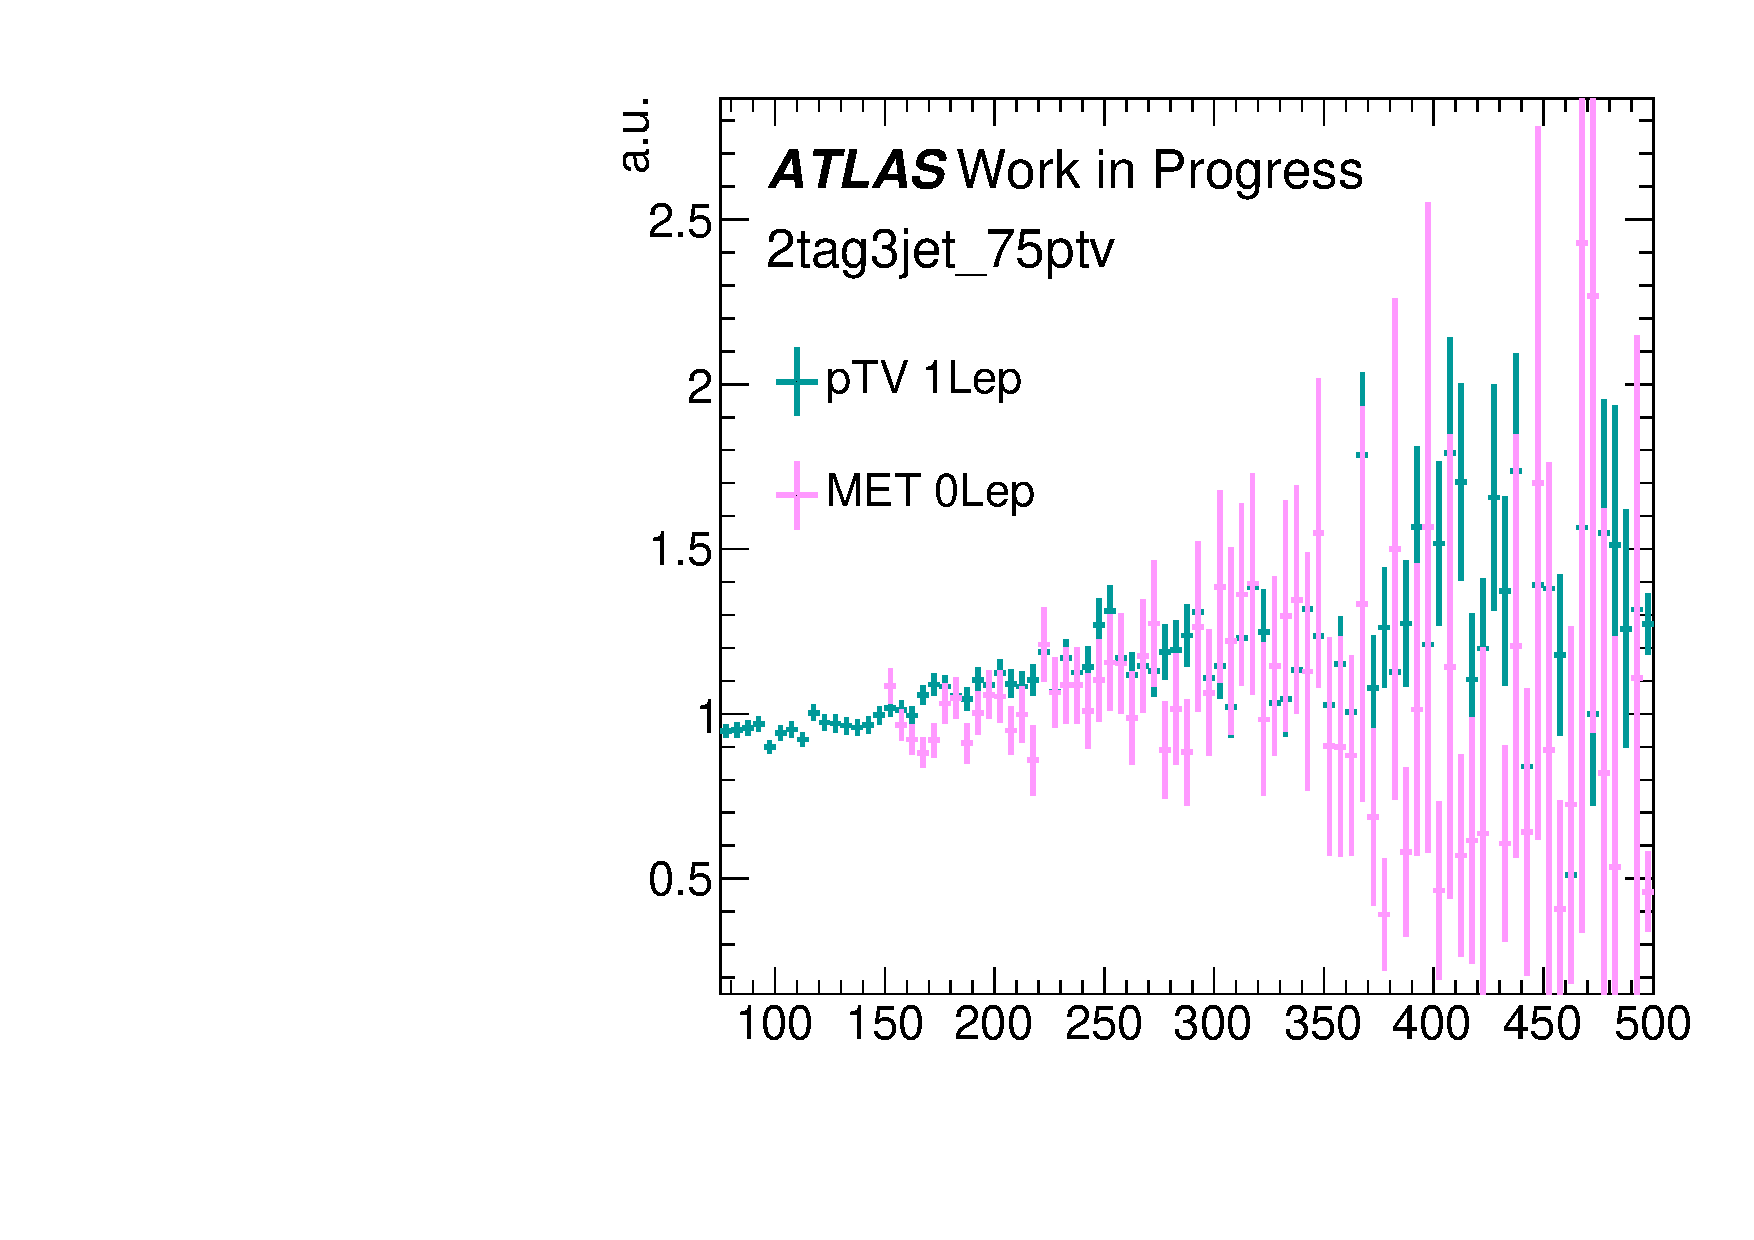
\includegraphics[width=0.45\textwidth]{figures/modelling_vjets/BDTreweighting/01Lep_reweighting_shapes/ReweightingVarComparison_2tag3jet_75ptv_bb.pdf}}
% \subfigure[2tag 3jet
% bc]{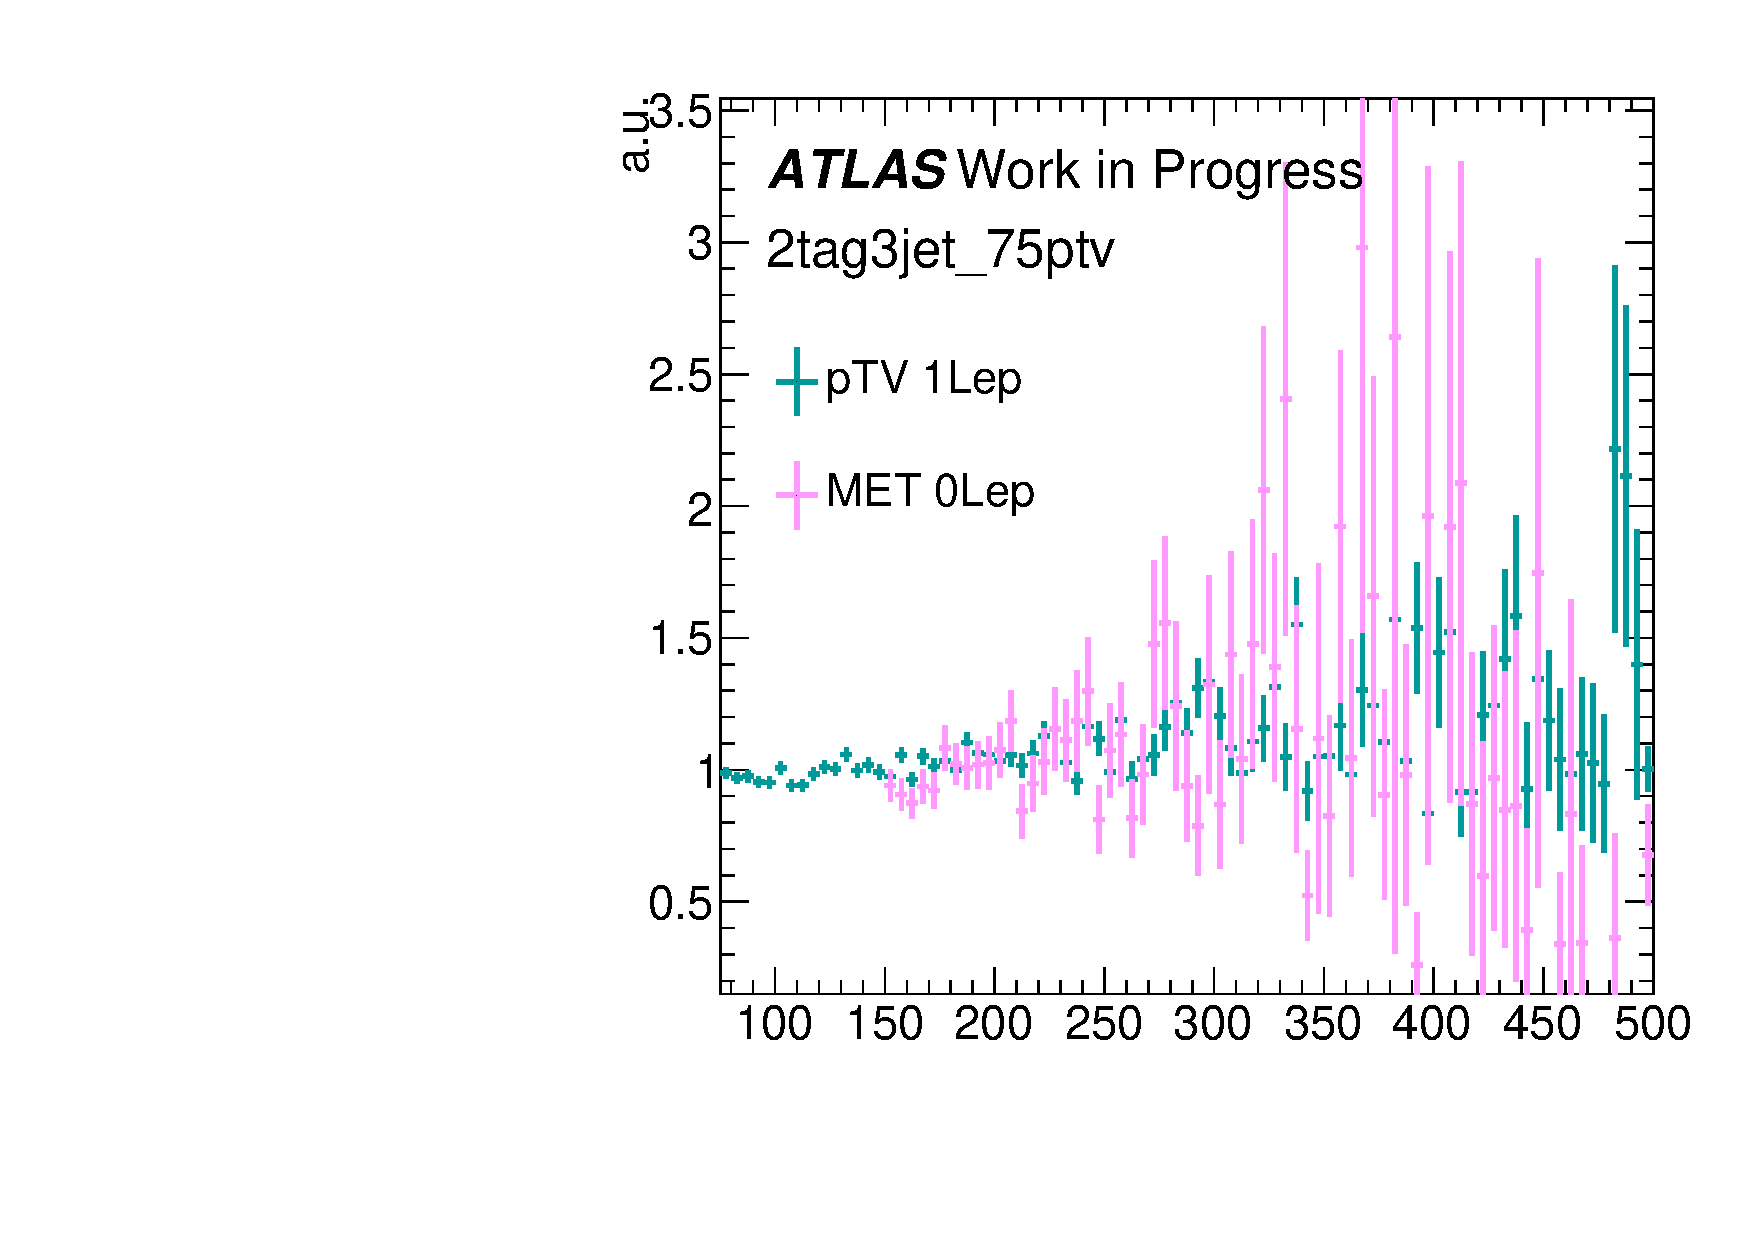
\includegraphics[width=0.45\textwidth]{figures/modelling_vjets/BDTreweighting/01Lep_reweighting_shapes/ReweightingVarComparison_2tag3jet_75ptv_bc.pdf}}
% \\
% \subfigure[2tag 3jet
% bl]{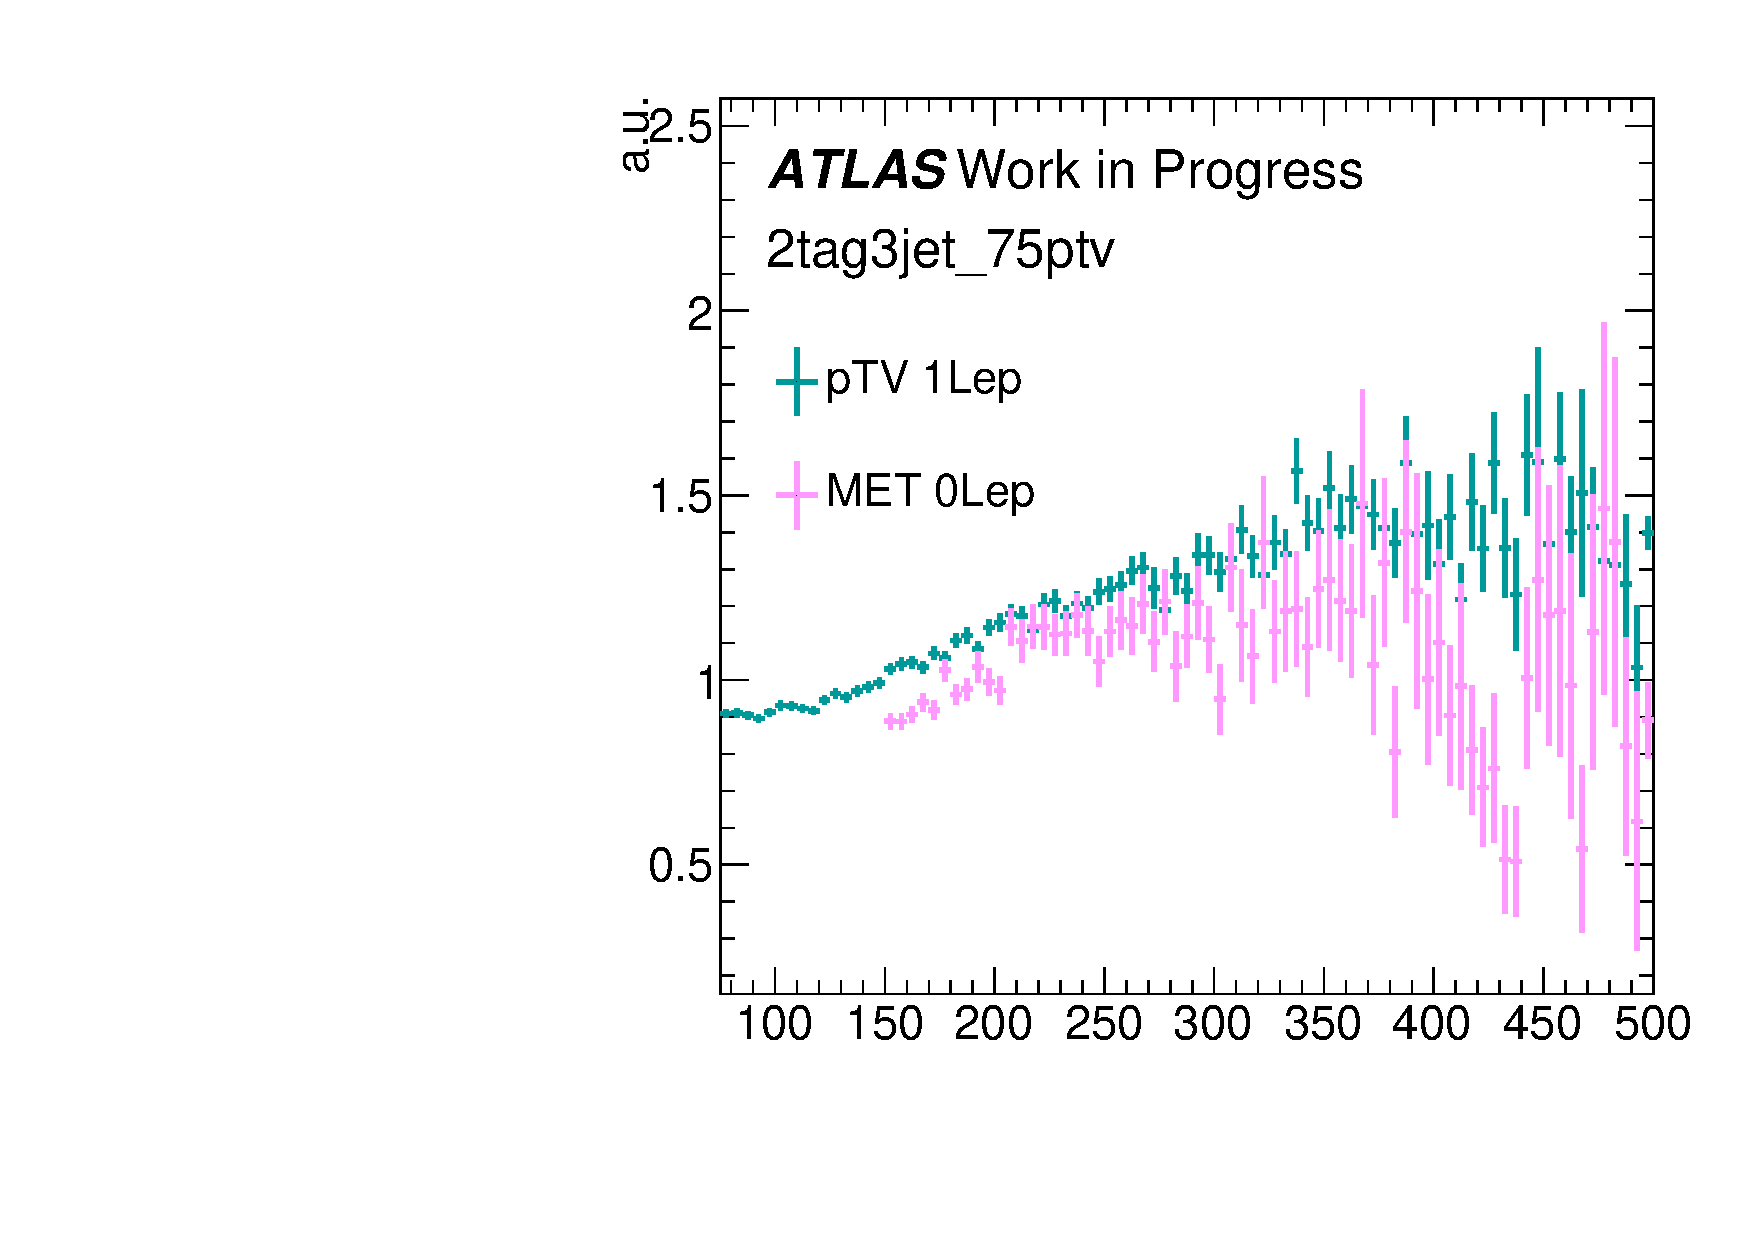
\includegraphics[width=0.45\textwidth]{figures/modelling_vjets/BDTreweighting/01Lep_reweighting_shapes/ReweightingVarComparison_2tag3jet_75ptv_bl.pdf}}
% \subfigure[2tag 3jet
% cc]{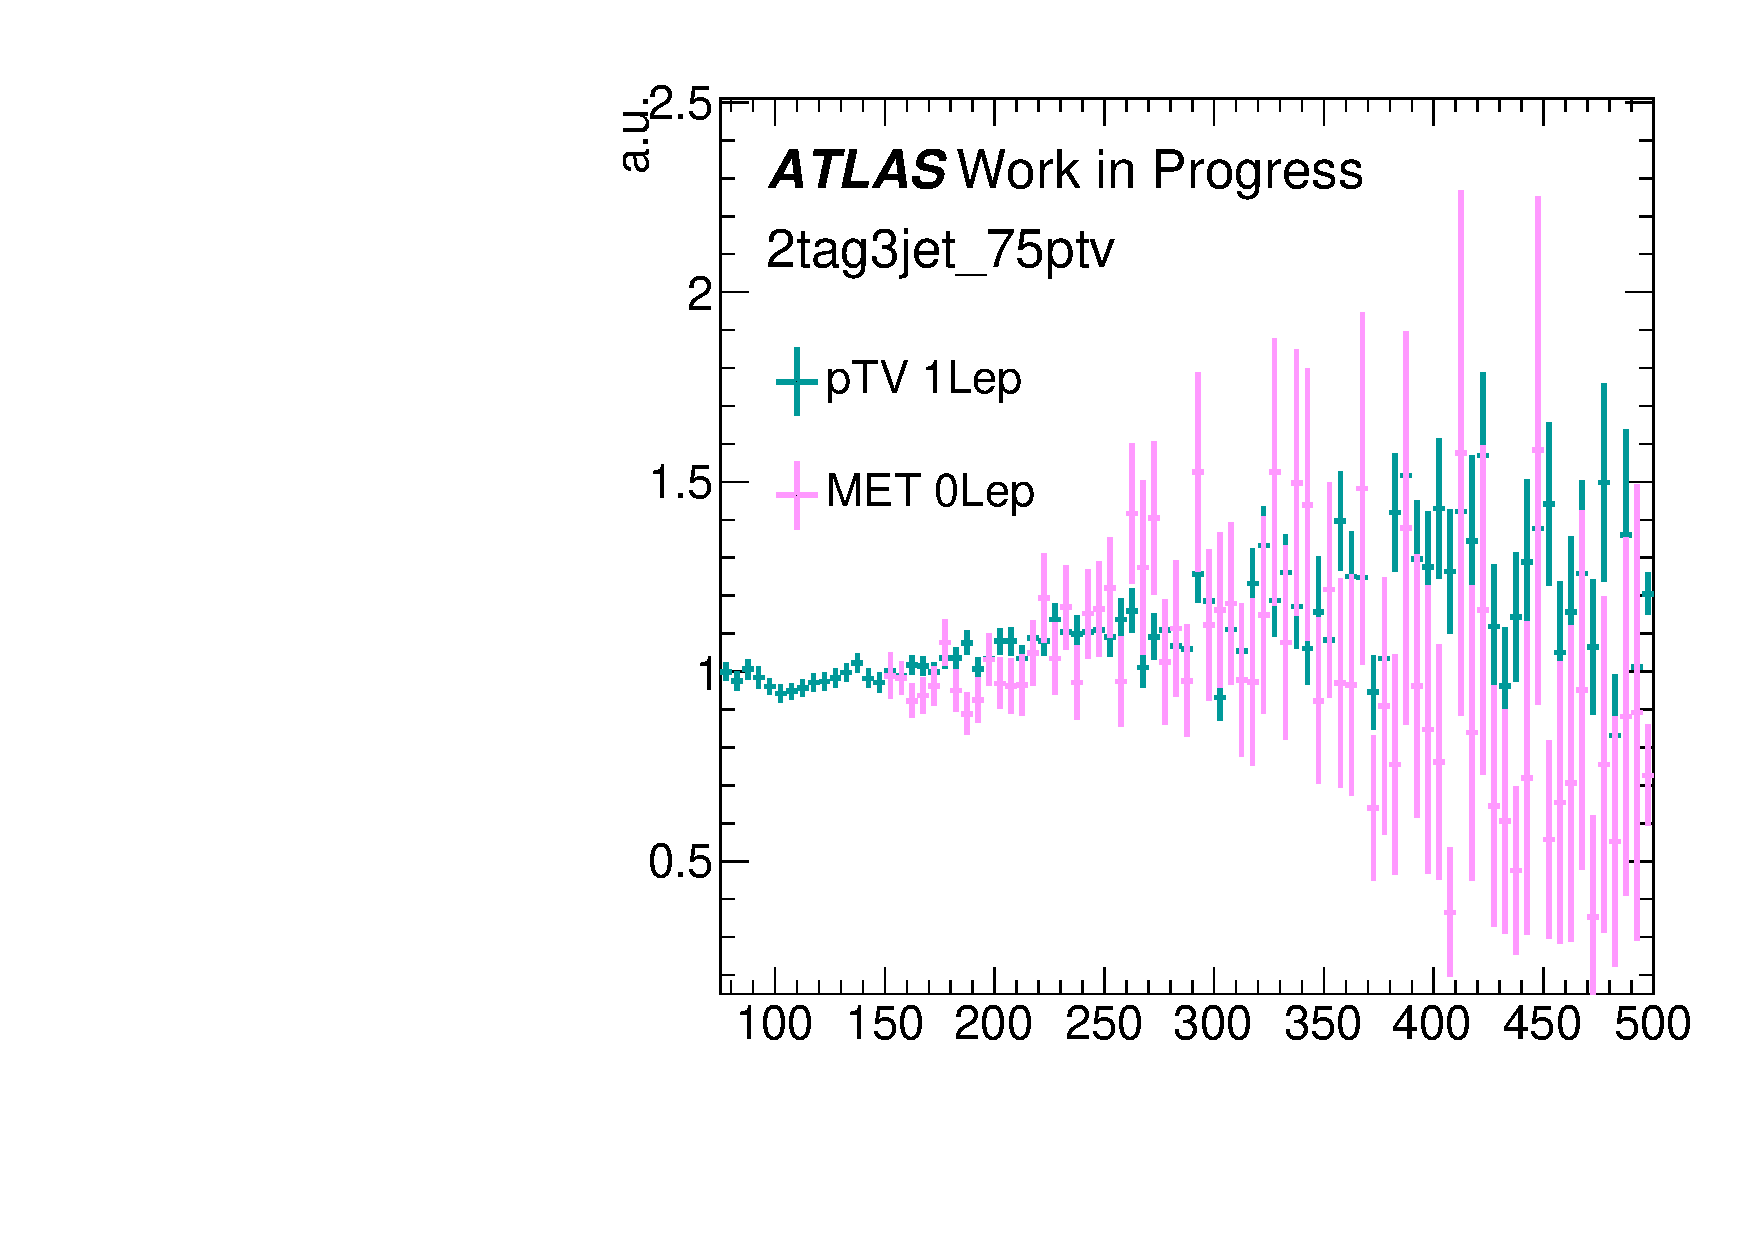
\includegraphics[width=0.45\textwidth]{figures/modelling_vjets/BDTreweighting/01Lep_reweighting_shapes/ReweightingVarComparison_2tag3jet_75ptv_cc.pdf}}
% \\
% \caption{$p_T^V$ and MET shape systematics derived in the 2tag3jet region of the
%   1-lepton and 0-lepton channels, respectively, for each heavy flavour pair.}
% \label{fig:wjets_01lep_3jet_SysWPtVBDTr}
% \end{center}
% \end{figure}

% \begin{figure}[H]
% \begin{center}
% \subfigure[$p_T^V$ and $MET$ 2tag 3jet
% bl]{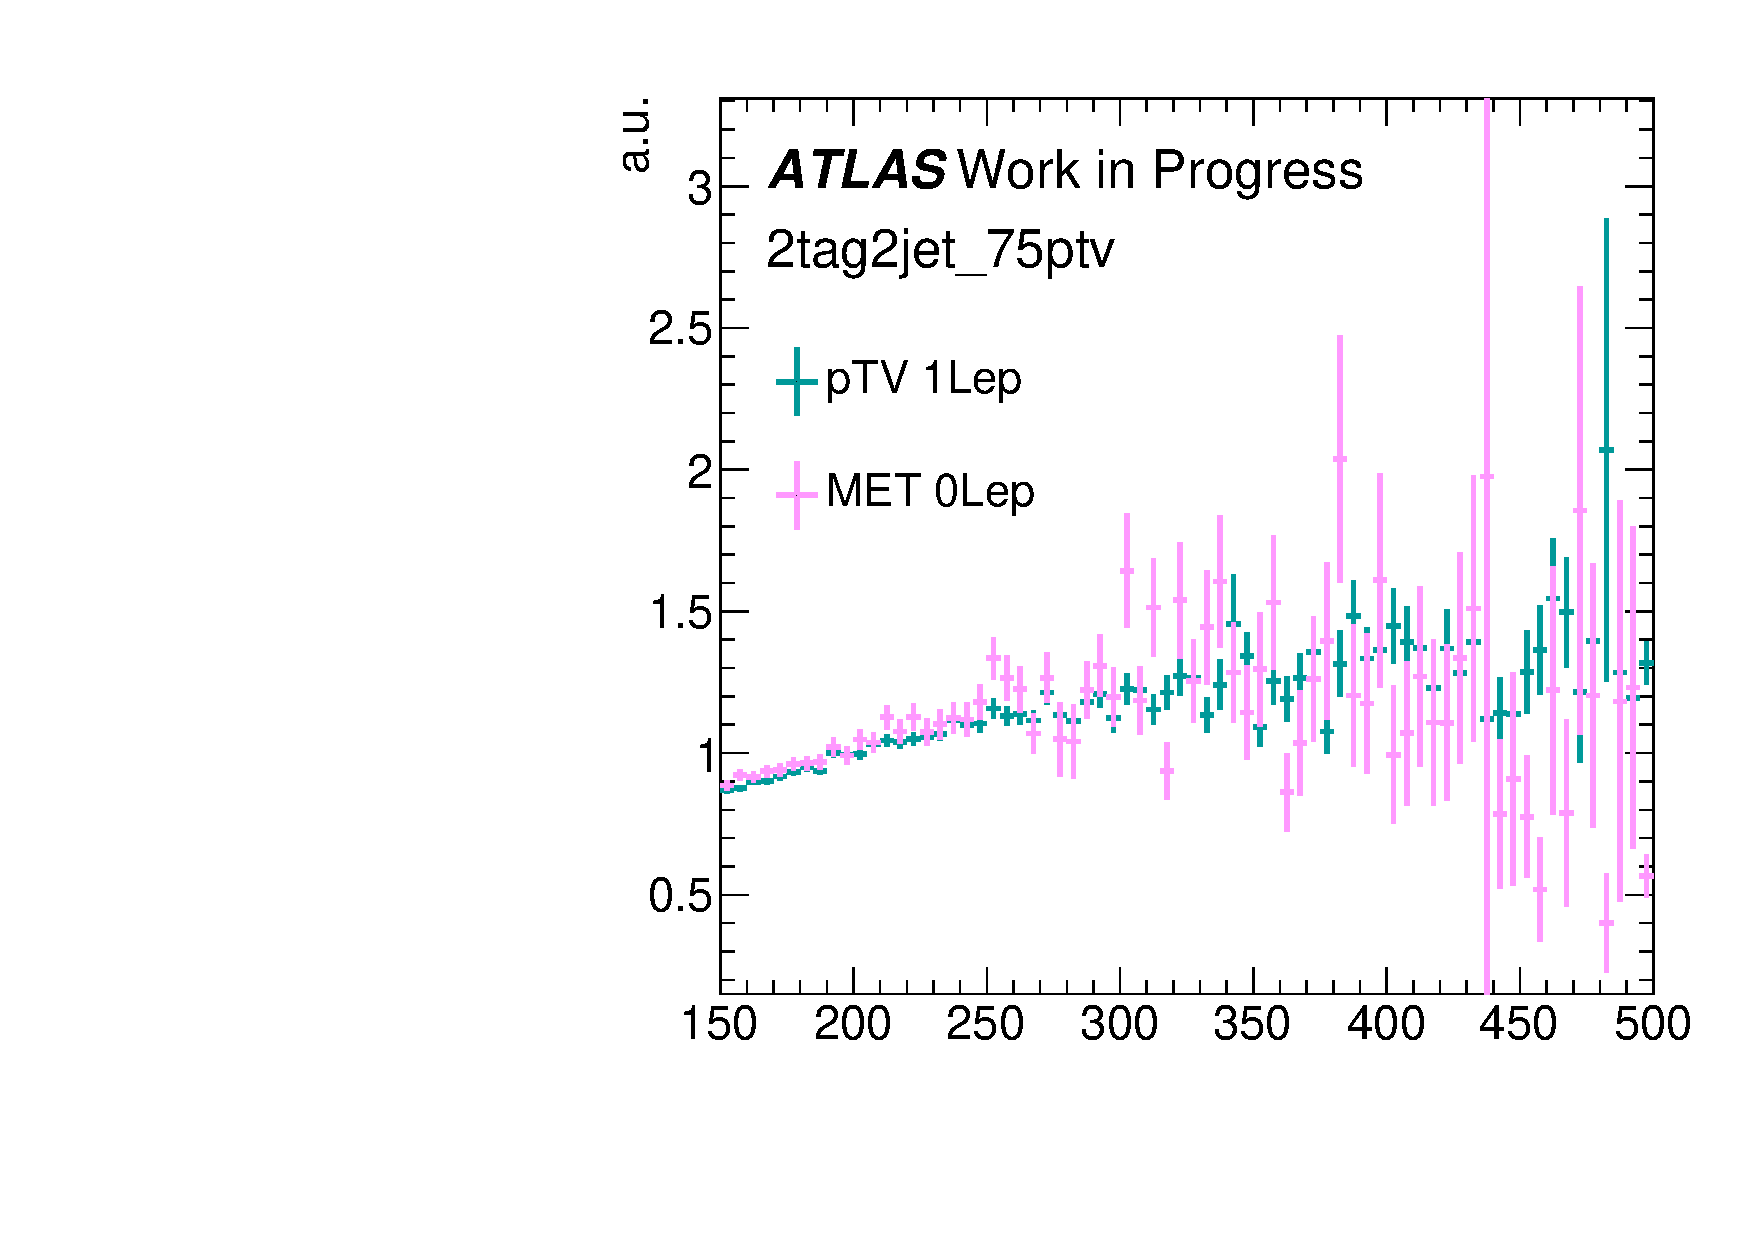
\includegraphics[width=0.45\textwidth]{figures/modelling_vjets/BDTreweighting/01Lep_reweighting_shapes/ReweightingVarComparison_2tag2jet_75ptv_bl_NormalizedFrom150.pdf}}
% \caption{$p_T^V$ and MET shape systematics derived in the 2tag2jet region of the
%   1-lepton and 0-lepton channels, respectively, for $W$+bl events, both
%   normalized in the $p_T^V > 150$\GeV and MET$ > 150$\GeV.}
% \label{fig:wjets_01lep_2jet_bl_SysWPtVBDTr_From150}
% \end{center}
% \end{figure}

% The $p_T^V$ shape systematic, derived in the 1-lepton channel, are thus applied to
% both the 1-lepton and the 0-lepton channel and implemented in the fit as a
% single nuisance parameter called \texttt{SysWPtV\_BDTr}.


\section{Experimental Systematics}
\begin{longtabu}{XX}
  \caption[A summary of experimental systematic uncertainties.]{A summary of the
    experimental systematic uncertainties considered in the analysis. They are
    listed by the name of the nuisance parameter entering into the
    profile-likelihood fit and a short description is provided of each
    uncertainty.}
  \label{tab:expSyst}\\
  \toprule
  {\bfseries Systematic uncertainty} & {\bfseries Short description} \\
  \midrule
  \endfirsthead
  \toprule
  {\bfseries Systematic uncertainty} & {\bfseries Short description} \\
  \midrule
  \endhead
  \midrule
  \multicolumn{2}{c}{Continued}\\   \bottomrule
  \endfoot
  \bottomrule
  \endlastfoot
  {\bfseries Event} & \\
  Luminosity & uncertainty on total integrated luminosity \\
  Pileup Re-weighting & uncertainty on pileup re-weighting \\
  {\bfseries Triggers} & \\
  \texttt{EL\_EFF\_Trigger\_Total\_1NPCOR\_PLUS\_UNCOR} &  electron trigger efficiency uncertainty\\
  \texttt{MUON\_EFF\_TrigStatUncertainty} &  \multirow{2}{*}{muon trigger efficiency uncertainty} \\
  \texttt{MUON\_EFF\_TrigSystUncertainty} & \\
  \texttt{METTrigStat}  &  \multirow{2}{*}{$E_{\mathrm{T}}^{\text{miss}}$trigger efficiency uncertainty} \\
  \texttt{METTrigTop/Z} & \\
  \texttt{METTrigSumpt} & \\
  {\bfseries Electrons}&\\%&\\
  \texttt{EL\_EFF\_Reco\_Total\_1NPCOR\_PLUS\_UNCOR} &  reconstruction efficiency uncertainty \\
  \texttt{EL\_EFF\_ID\_Total\_1NPCOR\_PLUS\_UNCOR} &  ID efficiency uncertainty \\
  \texttt{EL\_EFF\_Iso\_Total\_1NPCOR\_PLUS\_UNCOR} &  isolation efficiency uncertainty \\
  \texttt{EG\_SCALE\_ALL} &        energy scale uncertainty \\
  \texttt{EG\_RESOLUTION\_ALL} &    energy resolution uncertainty \\
  {\bfseries Muons}&\\
  \texttt{MUON\_EFF\_RECO\_STAT} &  \multirow{2}{*}{reconstruction and ID efficiency uncertainty for muons with $p_{\mathrm{T}}$\ $>$ 15 \GeV} \\
  \texttt{MUON\_EFF\_RECO\_SYS} &  \\
  \texttt{MUON\_EFF\_RECO\_STAT\_LOWPT} & \multirow{2}{*}{reconstruction and ID efficiency uncertainty for muons with $p_{\mathrm{T}}$\ $<$ 15 \GeV} \\
  \texttt{MUON\_EFF\_RECO\_SYS\_LOWPT} &  \\
  \texttt{MUON\_EFF\_TTVA\_STAT} &  \multirow{2}{*}{track-to-vertex association efficiency uncertainty} \\
  \texttt{MUON\_EFF\_TTVA\_SYS} &                      \\
  \texttt{MUON\_ISO\_STAT} &  \multirow{2}{*}{isolation efficiency uncertainty} \\
  \texttt{MUON\_ISO\_SYS} &                     \\
  \texttt{MUON\_ID} & momentum resolution uncertainty from inner detector        \\
  \texttt{MUON\_MS} &  momentum resolution uncertainty from muon system        \\
  \texttt{MUON\_SCALE} &   momentum scale uncertainty         \\
  \texttt{MUON\_SAGITTA\_RHO} & \multirow{2}{*}{charge dependent momentum scale uncertainty} \\
  \texttt{MUON\_SAGITTA\_RESBIAS} &  \\
  {\bfseries Jets and $\bm{b}$-tagging}&\\
  \texttt{JET\_CR\_JET\_EffectiveNP\_Detector1,2} & energy scale uncertainty from the in situ analyses (detector) \\
  \texttt{JET\_CR\_JET\_EffectiveNP\_Modelling1,...,4} & energy scale uncertainty from the in situ analyses (modelling) \\
  \texttt{JET\_CR\_JET\_EffectiveNP\_Statistical1,...,6} & energy scale uncertainty from the in situ analyses (stat) \\
  \texttt{JET\_CR\_JET\_EffectiveNP\_Mixed1,2,3} & energy scale uncertainty from the in situ analyses (mixed terms) \\
  \texttt{JET\_CR\_JET\_EtaIntercalibration\_Modeling} & energy scale uncertainty on eta-intercalibration (modelling)\\
  \texttt{JET\_CR\_JET\_EtaIntercalibration\_TotalStat} & energy scale uncertainty on eta-intercalibrations (statistics/method) \\
  \texttt{JET\_CR\_JET\_EtaIntercalibration\_NonClosure\_highE} & \multirow{3}{*}{energy scale uncertainty on eta-intercalibrations (non-closure)} \\
  \texttt{JET\_CR\_JET\_EtaIntercalibration\_NonClosure\_negEta} &\\
  \texttt{JET\_CR\_JET\_EtaIntercalibration\_NonClosure\_posEta} &\\
  \texttt{JET\_CR\_JET\_BJES\_Response} &  \\
  \texttt{JET\_CR\_JET\_Flavor\_Composition} & energy scale uncertainty on $V\!V$ and \VH\ sample's flavour composition \\
  & {$\rightarrow$ Independent NP for : "\texttt{\_Top}", "\texttt{\_Vjets}", "\texttt{\_VV}" processes } \\
  \texttt{JET\_CR\_JET\_Flavor\_Response} & energy scale uncertainty on samples' flavor response \\
  \texttt{JET\_CR\_JET\_Pileup\_OffsetMu} & energy scale uncertainty on pile-up (Mu dependent) \\
  \texttt{JET\_CR\_JET\_Pileup\_OffsetNPV} & energy scale uncertainty on pile-up (NPV dependent) \\
  \texttt{JET\_CR\_JET\_Pileup\_PtTerm} & energy scale uncertainty on pile-up (pt term) \\
  \texttt{JET\_CR\_JET\_Pileup\_RhoTopology} & energy scale uncertainty on pile-up (density $\rho$) \\
  \texttt{JET\_CR\_JET\_PunchThrough\_MC16} & energy scale uncertainty for punch-through jets \\
  \texttt{JET\_CR\_JET\_SingleParticle\_HighPt} & energy scale uncertainty from the behavior of high-pT jets \\
  \texttt{JET\_CR\_JET\_JER\_EffectivNP\_1,...6,7restTerm} & energy resolution uncertainty split into 7 components \\
  \texttt{JET\_CR\_JET\_JER\_DataVsMC} & energy resolution additional uncertainty difference between data than MC resolutions \\
  \texttt{JET\_JvtEfficiency} & JVT efficiency uncertainty \\
  \texttt{FT\_EFF\_Eigen\_B0,...,45} & \multirow{3}{*}{\parbox{11cm}{$b$-tagging efficiency uncertainties (``BTAG\_LOOSE'') in continuous mode: 45 components for $b$ jets, 20 for $c$ jets and 20 for light jets}} \\
  \texttt{FT\_EFF\_Eigen\_C0,...,20} &\\
  \texttt{FT\_EFF\_Eigen\_L0,...,20} &\\
  \texttt{FT\_EFF\_Eigen\_extrapolation} & $b$-tagging efficiency uncertainty on the extrapolation to high-$p_{\mathrm{T}}$\ jets \\
  \texttt{FT\_EFF\_Eigen\_extrapolation\_from\_charm} & $b$-tagging efficiency uncertainty on tau jets \\
  {\bfseries $\bm{E}_{\mathrm{T}}^{\text{miss}}$}&\\
  \texttt{MET\_SoftTrk\_ResoPara} & track-based soft term related longitudinal resolution uncertainty \\
  \texttt{MET\_SoftTrk\_ResoPerp} &  track-based soft term related transverse resolution uncertainty \\
  \texttt{MET\_SoftTrk\_Scale} & track-based soft term related longitudinal scale uncertainty \\
  \texttt{MET\_JetTrk\_Scale} & track MET scale uncertainty due to tracks in jets \\
  {\bfseries Taus}&\\
  \texttt{TAUS\_TRUEHADTAU\_SME\_TES\_DETECTOR} & energy scale uncertainty: single-particle response + threshold \\
  \texttt{TAUS\_TRUEHADTAU\_SME\_TES\_INSITU} & energy scale uncertainty: total from in-situ measurement \\
  \texttt{TAUS\_TRUEHADTAU\_SME\_TES\_MODEL} & energy scale uncertainty: modelling + closure \\
  \bottomrule
\end{longtable}

\section{V + jets systematics}
\label{sec:zjets-shapes}
Whilst the physics of the W and Z + jets processes leads to them being in
different channels and needing to be treated differently in the analysis, the
underlying theory means that simulation of these processes is coupled,
particularly as they are simulated with the same software.

The V + jets processes are simulated with
\textsc{Sherpa}~2.2.1~\cite{1126-6708-2009-02-007} as mentioned in
section~\ref{sec:composition}, which is interfaced with the
NNPDFs~\cite{Ball:2012cx} for both the matrix element calculation and the parton shower
tuning. Events with many additional jets produced in association with the vector
boson largely contribute to the background in this analysis, therefore a feature
of \textsc{Sherpa}~2.2.1 is used in which it provides a combination of matrix
elements with different parton multiplicities. Up to 2 extra partons are
included in the next-to-leading order matrix element, and 3 or 4 extra partons
are included at leading order in QCD. In order to combine different patron
multiplicities a matching scheme based on the CKKW-L~\cite{Lonnblad:2001iq,
  Lavesson:2005xu} merging technique is used, with a merging scale of $Q_{cut} =
20$~\GeV. Simulation of events with more than 4 extra partons relies on the
parton shower algorithm of \textsc{Sherpa}. The parton shower and underlying
events models are included in \textsc{Sherpa} whose generator adopts a full
5--flavour scheme with b- and c-quarks being treated as massless in the matrix
element, in the version used. Massive quarks can be produced in the parton
shower and heavy flavours (quarks as heavy or heavier than a c-quark) can be
produced directly in the scattering process of the underlying event.

The analysis gains a lot of sensitivity from high $p_T^V$ regions of phase
space, and also has the requirement of two b-tagged jets in the event selection
as mentioned in section~\ref{sec:selection}. It is therefore important to ensure
that a large statistical sample in these regions is available such that
fluctuations are smaller than those that would be found in the data. In order to
achieve this two methods are used, firstly samples are simulated in specific
slices of the larger of the $p_T$ of the vector boson or the $H_T$ of the event.
Events are simulated in the following slices
\begin{equation}
  \text{max}(p_T^V, H_T) = [0\text{--}70, 70\text{--}140, 140\text{--}280, 280\text{--}500, 500\text{--}1000, >1000]~\GeV.
\end{equation}
The dedicated slices at high $\text{max}(p_T^V, H_T)$ ensure a large number of
events are simulated in the high $p_T^V$ region of phase space. Secondly filters
are applied on the flavour of the jets that produced in association with the
vector boson.  The filters used for these samples are shown in
table~\ref{tab:bc-filters}.
\begin{table}[!htb]
  \centering
  \resizebox{0.95\textwidth}{!}{
    \begin{tabular}{lll}
      \toprule
      {\bfseries Filter} & {\bfseries Description} \\
      \midrule
      $b$-filter & at least 1 $b$-hadron with $p_{\mathrm{T}} >$0~GeV and $|\eta|<$4 \\
                         & at least 1 $b$-hadron with $p_{\mathrm{T}} >$5~GeV and $|\eta|<$2.9$^{\dagger}$ \\
      $c$-filter-$b$-veto & at least 1 $c$-hadron with $p_{\mathrm{T}}>$4~GeV and $|\eta|<$3   \\
                         & veto events which pass the $b$-filter  \\
      $c$-veto-$b$-veto & veto events which pass the $b$-filter or the $c$-filter-$b$-veto  \\
      \bottomrule
    \end{tabular}
  }
  \caption{Flavour filters used in the simulation of $V+$jets events. $\dagger$
    this tighter filter is only applied to $Z\to\nu\nu$ samples.}
  \label{tab:bc-filters}
\end{table}
The filters are not applied to the highest slices in $\text{max}(p_T^V, H_T)$.
The filtering strategy for $Z\nu\nu$ samples differs in the mc16e campaign using
a combination of $p_T^Z$ and $m_{jj}$ to better populate the region above the
MET trigger thresholds, and VBF phase spaces with high $m_{jj}$. These samples
also use a tighter b-filter compared to their mc16a/d counterpart which is also
described in table~\ref{tab:bc-filters}. All nominal V + jets samples with the
corresponding max($H_T$,$p_T^V$) slices and flavour filters are listed in
tables~\ref{tabular:mc_samples_Wjets} \ref{tabular:mc_samples_Zlljets}, and
\ref{tabular:mc_samples_Zvvjets} in the appendices.

A set of alternative predictions are used for a number of purposes in the
analysis, one such purpose is to investigate any discrepancies that may arise
between data and the nominal prediction. If the same discrepancy is present when
comparing he alternative prediction to data then the discrepancy may arise from
experimental error rather than weaknesses in the modelling. One kind of
modelling uncertainty also relies on the comparison of two predictions, for
example the nominal versus the alternative.

The alternative samples are generated using
\textsc{MadGraph}~5~\cite{MADGRAPH5_aMC@NLO} interfaced to \textsc{Pythia}~8 for
the modelling of the parton shower and the underlying event. The
\textsc{MadGraph}~5 v2 generator provides a LO (QCD) description of these
processes, merging together matrix-element calculations with different parton
multiplicities, up to 4 additional jets, higher jet multiplicities are modelled
by the parton shower algorithm. The merging scheme applied to combine different
parton multiplicities is the same as for the nominal samples, the CKKW-L scheme,
but has a merging scale of $Q_{cut} = 30$~\GeV. For the LO ME calculation the
NNPDF2.3 LO PDFs are used, with $\alpha_S = 1.3$.  Similarly to
\textsc{Sherpa}~2.2.1, also \textsc{MadGraph}~adopts a full 5-flavour scheme
with massless quarks in the ME calculation, while massive quarks can be produced
by the parton shower. All alternative V + jets samples are listed in
tables~\ref{tabular:zjetsAlternativeSamples} and
\ref{tabular:wjetsAlternativeSamples} in the appendices.

As well as using an alternative Monte-Carlo generator the nominal generator,
\textsc{Sherpa}, includes systematic variations internally. Every
\textsc{Sherpa}~2.2.1 V + jets sample has an event weight corresponding to each
of the variations detailed in table~\ref{tab:sherpa-variations}\footnote{Some of
the variations cannot be produced by \textsc{Sherpa}~2.2.1 and so
\textsc{Sherpa}~2.1 is used instead. For these variations half of the variation
in each direction is taken as the uncertainty rather than comparing to the
central value of the \textsc{Sherpa}~2.2.1 prediction.}.
\begin{table}
  \centering
  \begin{tabular}{ l l l }
    \toprule
    \bfseries{Variation} & \multicolumn{2}{l}{\bfseries{Values}} \\
    \midrule
    \multicolumn{3}{l}{\bfseries{Sherpa 2.2.1}} \\
    Factorisation scale ($\mu_F$) & $2\mu_F$ & 0.5$\mu_F$ \\
    Renormalisation scale ($\mu_R$) & $2\mu_R$ & 0.5$\mu_R$ \\
    PDF Variation & MMHT2014nnlo68cl & CT14nnlo \\
    &&\\
    \multicolumn{3}{l}{\bfseries{Sherpa 2.1}} \\
    Re-summation scale ($\mu_S$) & $2\mu_S$ & 0.5$\mu_S$ \\
    CKKW Merging scale & 15 \GeV & 30 \GeV \\
    \bottomrule
  \end{tabular}
  \caption{A summary of the Sherpa 2.2.1 and Sherpa 2.1 internal variations that
  are used to model V + jets processes.}
  \label{tab:sherpa-variations}
\end{table}

\subsubsection{V + jets cross-section}
The V + jets cross sections are known at NNLO (QCD)~\cite{Butterworth:1287902},
the higher order cross sections are used to normalise the V+jets samples in the
analysis. For the W + jets samples the total cross section from \textsc{Sherpa} or
from \textsc{MadGraph}, averaged across all 3 lepton flavours taking into account the
different hadron filter efficiencies, is scaled to the NNLO prediction obtaining
scaling factor of $k_{\text{NNLO}}^{\text{QCD}} = 0.9702$.

For Z + jets some subtleties must be considered. For $Z \to \ell\ell$ + jets the
cut at generator level, $m_{\ell\ell}>40$ \GeV, must be taken into account. The
NNLO calculation uses a cut of $66<m_{\ell\ell}<116$ \GeV, which can be applied
at truth level to the samples of this analysis in order to get the scaling
correct as follows:
\begin{equation}
  k_{\text{NNLO}}^{\text{QCD}} = \frac{\sigma_{\text{NNLO}}(66<m_{\ell\ell}<116\,{\GeV})}{\sigma_{\textsc{Sherpa},\textsc{MadGraph}}(66<m_{\ell\ell}<116\,{\GeV})},
  \label{eq:nnlo-vjets-k}
\end{equation}
hence the scaling factor is found to be $0.9751$. For $Z \to \nu\nu$ +jets the
NNLO no theoretical cross section is available. Values from the
Particle Data Group (PDG)~\cite{PDG} are used to correct for the difference
between the BR($Z \to \nu\nu$) and BR($Z \to \ell\ell$), and the NNLO cross
section is used without any mass cuts and with the $Z/\gamma^*$ interference
removed. The scaling factor is therefore calculated to be $0.9728$. It is not
necessarily expected that the scaling factors should be different for $Z \to
\ell \ell$ and $Z \to \nu \nu$ events but this can be explained as both
\textsc{Sherpa} and \textsc{MadGraph} used different branching ratios for these
two processes in their generators compared with those used by the higher order
theoretical calculations.

\subsection{W + jets systematics}
\begin{table}
\resizebox{\textwidth}{!}{
  \begin{tabular}{lllll}
   \toprule
    {\bfseries Nuisance Parameter} & {\bfseries Descriptio}n & {\bfseries Samples/Categories} & {\bfseries Value} & {\bfseries Effect} \\
    \midrule
    \texttt{norm\_Wbb\_J2} 	& Floating $W hf$ norm $2$-jet events  	& $W hf$, $2$-jet categories    & Float	& Normalization\\ %\hline
    \texttt{norm\_Wbb\_J3} 	& Floating $W hf$ norm $3$(+)-jet events  	& $W hf$, $3$(+)-jet categories & Float	& Normalization\\ %\hline
    %% \texttt{norm\_Wbb\_J2\_Bmin75\_L1} 	& Floating $W hf$ norm in medium p_T^V ($75$ to $150$ \GeV) $2$-jet events  	& $W hf$, $2$-jet and $p_T^V\in[75,150]~\GeV$ categories & Float	& Normalization\\ %\hline
    %% \texttt{norm\_Wbb\_J3\_Bmin75\_L1} 	& Floating $W hf$ norm in medium p_T^V ($75$ to $150$ \GeV) $3$(+)-jet events  	& $W hf$, $3$(+)-jet and $p_T^V\in[75,150]~\GeV$ categories & Float	& Normalization\\ %\hline
    %% \texttt{norm\_Wbb\_J2} 	& Floating $W hf$ norm in high p_T^V ($>150~\GeV$) $2$-jet events  	& $W hf$, $2$-jet and $p_T^V>150~\GeV$ categories    & Float	& Normalization\\ %\hline
    %% \texttt{norm\_Wbb\_J3} 	& Floating $W hf$ norm in high p_T^V ($>150~\GeV$) $3$(+)-jet events  	& $W hf$, $3$(+)-jet and $p_T^V>150~\GeV$ categories & Float	& Normalization\\ %\hline
    \texttt{SysWlNorm} 	  & $Wl$ normalization          & $Wl$, all regions 	                                & 32\% 	&Normalization\\
    \texttt{SysWclNorm} 	  & $Wcl$ normalization         & $Wcl$, all regions 	                                & 37\% 	&Normalization\\
    \texttt{SysWbbNorm\_L0}& Uncertainty on 1- to 0-lep $W hf$ norm extrapolation & $W hf$ , 0--lepton channel                         & 5\%	&Normalization\\
    \texttt{SysWccWbbRatio}& $Wcc / Wbb$ ratio & $Wcc$, all regions & 26\% (0-l), 23\% (1-l) &Normalization\\        
    \texttt{SysWbcWbbRatio}& $Wbc / Wbb$ ratio & $Wbc$, all regions & 15\% (0-l), 30\% (1-l) &Normalization\\        
    \texttt{SysWblWbbRatio}& $Wbl / Wbb$ ratio & $Wcl$, all regions & 10\% (0-l), 30\% (1-l) &Normalization\\        
    \texttt{SysWbbCRSRextrap} & Uncertainty on SR to CRs $W$+jets extrapolation & W+jets, CRLow and CRHigh & 3.6\%-14.9\% &Normalization\\
    \texttt{SysWPtV\_J2}             & $p_T^V$\ shape & W + jets, $2$-jet regions & - & Migration+Shape \\
    \texttt{SysWPtV\_J3}             & $p_T^V$\ shape & W + jets, $3$-jet regions & - & Migration+Shape \\
    \texttt{SysBDTr\_W\_SHtoMG5}             & \textsc{Sherpa} to \textsc{MadGraph} mva shape from $p_T^V$-factorized BDTr method  & W + jets, all regions& - & Shape \\
    %% \texttt{SysWPtV\_J2}             & $p_T^V$\ shape & W + jets, $2$-jet, $p_T^V>150~\GeV$ regions & - & Normalization+Shape \\
    %% \texttt{SysWPtV\_J2\_Bmin75\_L1} & $p_T^V$\ shape & W + jets, $2$-jet, $p_T^V\in[75,150]~\GeV$ regions & - & Normalization+Shape \\
    %% \texttt{SysWPtV\_J3}             & $p_T^V$\ shape & W + jets, $3$-jet, $p_T^V>150~\GeV$ regions & - & Normalization+Shape \\
    %% \texttt{SysWPtV\_J3\_Bmin75\_L1} & $p_T^V$\ shape & W + jets, $3$-jet, $p_T^V\in[75,150]~\GeV$ regions & - & Normalization+Shape \\
    %% \texttt{SysBDTr\_W\_SHtoMG5}             & \textsc{Sherpa} to \textsc{MadGraph} mva shape from p_T^V-factorized BDTr method  & W + jets, $p_T^V>150~\GeV$ regions & - & Normalization+Shape \\
    %% \texttt{SysBDTr\_W\_SHtoMG5\_Bmin75\_L1} & \textsc{Sherpa} to \textsc{MadGraph} mva shape from p_T^V-factorized BDTr method  & W + jets, $p_T^V\in[75,150]~\GeV$ regions & - & Normalization+Shape \\
\bottomrule
\end{tabular}
}
\caption[Summary of $W+$jet specific nuisance parameters.]{Summary of the
  $W$+jets systematic uncertainties: the first column quotes the name of the
  nuisance parameter implemented in the fit referring to a specific systematic
  uncertainty, the second column the source of the uncertainty, the third the
  categories and sample on which it is applied, the fourth column the value of
  the Gaussian prior on the NP (if applicable) and the fifth column the effect
  of the systematic uncertainty. The listed systematic uncertainties are
  separated in normalization effects (first block), acceptance effects (second
  block), and shape systematic uncertainties (third block).}
\label{tab:Wjets_systematics}
\end{table}

\subsubsection{Normalisation and Acceptance Errors}

\subsubsection{Shape Errors}

\subsection{Z + jets systematics}

\begin{table}
\resizebox{\textwidth}{!}{
\begin{tabular}{lllll}
  \toprule
  {\bfseries Nuisance Parameter} & {\bfseries Description} & {\bfseries Samples/Categories} & {\bfseries Value} & {\bfseries Effect}  \\
  \midrule
  \texttt{norm\_Zbb\_J2\_Bmin75\_L2} 	& Floating $Z hf$ norm in medium $p_T^V$ ($75-150$ \GeV) $2$-jet events  	& $Z hf$, $2$-jet and $p_T^V\in[75,150[~\GeV$ vategory & Float	& Normalization\\ %\hline
  
  \texttt{norm\_Zbb\_J3\_Bmin75\_L2} 	& Floating $Z hf$ norm in medium $p_T^V$ ($75-150$ \GeV) $3$(+)-jet events  	& $Z hf$, $3$(+)-jet, $p_T^V\in[75,150[~\GeV$ category & Float	& Normalization\\ %\hline
  \texttt{norm\_Zbb\_J2} 	& Floating $Z hf$ norm in high $p_T^V$ ($>150~\GeV$) $2$-jet events  	& $Z hf$, all $2$-jet and $p_T^V>150~\GeV$ categories & Float	& Normalization\\ %\hline
  \texttt{norm\_Zbb\_J3} 	& Floating $Z hf$ norm in high $p_T^V$ ($>150~\GeV$) $3$(+)-jet events  	& $Z hf$, all $3$(+)-jet and $p_T^V>150~\GeV$ categories & Float	& Normalization\\ %\hline
  \texttt{SysZlNorm} 	  & $Zl$ normalization  & $Zl$, all regions 	                                        & 18\% 	& Normalization\\
  \texttt{SysZclNorm} 	  & $Zcl$ normalization & $Zcl$, all regions 	                                        & 23\% 	& Normalization\\
  \texttt{SysZbbNorm\_0L}& Uncertainty on $Z hf$ norm extrapolation to $0$-lep &  $Z hf$ normalization in 0--lepton & 7\% & Normalization\\
  \texttt{SysZccZbbRatio}& $Zcc / Zbb$ ratio & $Zcc$, all regions & 15\% (0-l), 16\% (2-l, 2-j), 13\% (2-j, 3+-j) & Normalization\\            
  \texttt{SysZbcZbbRatio}& $Zbc / Zbb$ ratio & $Zbc$, all regions & 40\% (0-l), 40\% (2-l, 2-j), 30\% (2-j, 3+-j) &Normalization\\        
  \texttt{SysZblZbbRatio}& $Zbl / Zbb$ ratio & $Zbl$, all regions & 25\% (0-l), 28\% (2-l, 2-j), 20\% (2-j, 3+-j) & Normalization\\        
  \texttt{SysZbbCRSRextrap\_BMin75\_L2\_CRLow} & Uncertainty on SR to CRLow $Z$+jets extrapolation & Z+jets, CRLow  $p_T^V\in[75,150[~\GeV$ & 3.8\%-9.9\% & Normalization\\        
  \texttt{SysZbbCRSRextrap\_BMin75\_L2\_CRHigh} & Uncertainty on SR to CRHigh $Z$+jets extrapolation & Z+jets, CRHigh $p_T^V\in[75,150[~\GeV$ & 2.7\%-4.1\% & Normalization\\        
  \texttt{SysZbbCRSRextrap\_CRLow} & Uncertainty on SR to CRLow $Z$+jets extrapolation & Z+jets, CRLow $p_T^V>150~\GeV$ & 3.8\%-9.9\% & Normalization\\        
  \texttt{SysZbbCRSRextrap\_CRHigh} & Uncertainty on SR to CRHigh $Z$+jets extrapolation & Z+jets, CRHigh $p_T^V>150~\GeV$ & 2.7\%-4.1\% & Normalization\\           
  \texttt{SysZPTV} & $p_T^V$\ shape & Z+jets, all regions with $p_T^V>150~\GeV$ & - & Migration+Shape \\
  \texttt{SysZPTV\_BMin75\_L2} & $p_T^V$\ shape & Z+jets, all regions in $p_T^V\in[75,150[~\GeV$ & - & Migration+Shape \\
  \texttt{SysZMbb} & $m_{bb}$\ shape & Z+jets, all regions with $p_T^V>150~\GeV$ & - & Shape \\
  \texttt{SysZMbb\_BMin75\_L2} & $m_{bb}$\ shape & Z+jets, all regions in $p_T^V\in[75,150[~\GeV$ & - & Shape \\
\bottomrule
\end{tabular}
}
\caption{Z + jets systs summary}
  % Summary of the Z +
  % jets systematic uncertainties: the first column quotes the name of the
  % nuisance parameter implemented in the fit referring to a specific systematic
  % uncertainty, the second column the source of the uncertainty, the third the
  % categories and sample on which it is applied, the fourth column the value of
  % the Gaussian prior on the NP (if applicable) and the fifth column the type of
  % systematic uncertainty. The listed systematic uncertainties are separated in
  % normalization effects (first block), acceptance effects (second block), and
  % shape systematic uncertainties (third block). %For details on the evaluation
  %                               %of these systematics see Sections 4.1.5, 4.1.6
  %                               %and 4.1.7 of
  %                               %Ref.\,\cite{VHmodellingsupportnote}.
\label{tab:Zjets_systematics}
\end{table}

\section{Top Quark Systematics}
\begin{table}[hbpt!]
  \resizebox{\textwidth}{!}{
    \begin{tabular}{lllll}
      \toprule
      {\bfseries Nuisance Parameter} & {\bfseries Description} & {\bfseries Categories} & {\bfseries Value}  \\
      \midrule
      {\bfseries Normalisation} & & & & \\
      \texttt{norm\_ttbar\_J2} & Floating $t\bar{t}$ norm     &  $t\bar{t}$, $0/1$--lepton, $2$--jet regions 	& Float	\\
      \texttt{norm\_ttbar\_J3} & Floating $t\bar{t}$ norm     &  $t\bar{t}$, $0/1$--lepton, $3$--jet regions 	& Float	\\
      {\bfseries Acceptance} & & &  \\
      \texttt{SysTTbarNorm\_L0} &  1-- to 0--lep $t\bar{t}$ norm extrapolation     &  0--lepton 	& 8\%	\\
      {\bfseries Flavour Composition}  & & & \\ 
      \texttt{SysTTbarbcMeACC} &  $bc/bb$ acceptance ratio from ME variation & $0/1$--lepton channels & - \\
      \texttt{SysTTbarbcPSACC} &  $bc/bb$ acceptance ratio from PS variation & $0/1$--lepton channels & - \\
      \texttt{SysTTbarOthMeACC} &  $\text{Oth}/bb$ acceptance ratio from ME variation & $0/1$--lepton channels & - \\
      \texttt{SysTTbarOthPSACC} &  $\text{Oth}/bb$ acceptance ratio from PS variation & $0/1$--lepton channels & - \\
      {\bfseries Shape} & & &  \\ 
      \texttt{SysTTbarPtV\_J2} & 0+1--lep $p_{\mathrm{T}}^V$\ shape & $0/1$--lepton channels, 2--jet regions & - \\
      \texttt{SysTTbarPtV\_J3} & 0+1--lep $p_{\mathrm{T}}^V$\ shape & $0/1$--lepton channels, 3--jet regions & - \\
      \texttt{SysBDTr\_ttbar\_ME\_J2} & \textsc{Powheg} to \textsc{MadGraph} multi-variate shape  & $0/1$--lepton channels, 2--jet regions & - \\
      \texttt{SysBDTr\_ttbar\_ME\_J3} & \textsc{Powheg} to \textsc{MadGraph} multi-variate shape & $0/1$--lepton channels, 3--jet regions & - \\
      \texttt{SysBDTr\_ttbar\_PS\_L0} & \textsc{Pythia8} to \textsc{Herwig7} multi-variate shape  & $0$--lepton channel & - \\
      \texttt{SysBDTr\_ttbar\_PS\_Bmin150\_L1} & \textsc{Pythia8} to \textsc{Herwig7} multi-variate shape  & $1$--lepton channel, $150~\GeV< p_{\mathrm{T}}^V <250~\GeV$ & - \\
      \texttt{SysBDTr\_ttbar\_PS} & \textsc{Pythia8} to \textsc{Herwig7} multi-variate shape  & $1$--lepton channel, rest & - \\
      \bottomrule
    \end{tabular}
  }
  \caption[A summary of systematic uncertainties on $t\bar{t}$ events.]{A
    summary of systematic uncertainties of $t\bar{t}$ events. Uncertainties are
    listed by the nuisance parameter that controls them in the profile-likelihood
    fit, a short description is provided for each and the categories in which the
    uncertainty are applied are shown. If a prior is calculated it's value is
    listed. All uncertainties in this table except those under normalisation are
    allowed to affect both the yield and shape of distributions.}
  \label{tab:ttbar-systs}
\end{table}

\subsubsection{Normalisation and Acceptance Errors}

\subsubsection{Shape Errors}

\section{Small background systematics}
\begin{table}
  \resizebox{\textwidth}{!}{
    \begin{tabular}{lllll}
      \toprule
      {\bfseries Nuisance Parameter} & {\bfseries Description} & {\bfseries Categories} & {\bfseries Value} & {\bfseries Effect}  \\
      \midrule
      {\bfseries Multi-jet}&&&\\
      \texttt{SysMJNorm\_2J\_El}    & multi-jet normalization 	&  1--lepton channel, 2-jet, $e$ 	& +200\% - 100\% 	&Normalization\\
      \texttt{SysMJNorm\_3J\_El}    & multi-jet normalization 	&  1--lepton channel, 3-jet, $e$ 	& +100\% - 100\% 	&Normalization\\
      \texttt{SysMJNorm\_2J\_Mu}    & multi-jet normalization 	&  1--lepton channel, 2-jet, $\mu$       & +47\% -  29\% 	&Normalization\\
      \texttt{SysMJNorm\_3J\_Mu}    & multi-jet normalization 	&  1--lepton channel, 3-jet, $\mu$       & +100\% - 100\% 	&Normalization\\
      %% \texttt{SysMJNorm\_2J\_El}    & multi-jet normalization 	&  1--lepton channel, 2-jet, $e$, $$p_T^V$>150~\GeV$		& +200\% - 100\% 	&Normalization\\
      %% \texttt{SysMJNorm\_2J\_El\_BMin75}   & multi-jet normalization 	&  1--lepton channel, 2-jet, $e$, $$p_T^V$\in[75,150]~\GeV$		& +200\% - 100\% 	&Normalization\\
      %% \texttt{SysMJNorm\_3J\_El}    & multi-jet normalization 	&  1--lepton channel, 3-jet, $e$, $$p_T^V$>150~\GeV$		& +100\% - 100\% 	&Normalization\\
      %% \texttt{SysMJNorm\_3J\_El\_BMin75}   & multi-jet normalization 	&  1--lepton channel, 3-jet, $e$, $$p_T^V$\in[75,150]~\GeV$		& +100\% - 100\% 	&Normalization\\
      %% \texttt{SysMJNorm\_2J\_Mu}    & multi-jet normalization 	&  1--lepton channel, 2-jet, $\mu$, $$p_T^V$>150~\GeV$	        & +47\% -  29\% 	&Normalization\\
      %% \texttt{SysMJNorm\_2J\_Mu\_BMin75}   & multi-jet normalization 	&  1--lepton channel, 2-jet, $\mu$, $$p_T^V$\in[75,150]~\GeV$	& +47\% -  29\% 	&Normalization\\
      %% \texttt{SysMJNorm\_3J\_Mu}    & multi-jet normalization 	&  1--lepton channel, 3-jet, $\mu$, $$p_T^V$>150~\GeV$	        & +100\% - 100\% 	&Normalization\\
      %% \texttt{SysMJNorm\_3J\_Mu\_BMin75}  & multi-jet normalization 	&  1--lepton channel, 3-jet, $\mu$, $$p_T^V$\in[75,150]~\GeV$	& +100\% - 100\% 	&Normalization\\
      % \texttt{SysMJTrigger} & multi-jet shape & 1--lepton, electron channel & - & Shape \\
      \texttt{SysMJReduced} & multi-jet shape change with isolation criteria & 1--lepton, $e$ and $\mu$ channel & - & Shape \\
      \texttt{SysMJSFsCR} & multi-jet shape change with $W +$HF/Top scaling & 1--lepton, $e$ and $\mu$ channel & - & Shape \\
      %% \texttt{SysMJReduced} & multi-jet shape change with isolation criteria & 1--lepton, $e$ and $\mu$ channel, $$p_T^V$>150~\GeV$ & - & Shape \\
      %% \texttt{SysMJReduced\_BMin75} & multi-jet shape change with isolation criteria & 1--lepton, $e$ and $\mu$ channel, $$p_T^V$\in[75,150]~\GeV$ & - & Shape \\
      %% \texttt{SysMJSFsCR} & multi-jet shape change with $W +$HF/Top scaling & 1--lepton, $e$ and $\mu$ channel, $$p_T^V$>150~\GeV$ & - & Shape \\
      %% \texttt{SysMJSFsCR\_BMin75} & multi-jet shape change with isolation criteria & 1--lepton, $e$ and $\mu$ channel, $$p_T^V$\in[75,150]~\GeV$ & - & Shape \\
      {\bfseries Single top}&&&&\\
      \texttt{stopsNorm}    & single-top ($s$-channel) normalization 	&  all regions	& 4.6\%	&Normalization\\
      \texttt{stoptNorm}    & single-top ($t$-channel) normalization 	&  all regions	& 4.4\%	&Normalization\\
      \texttt{stopWtNorm}   & single-top ($Wt$-channel) normalization &  all regions	& 6.2\%	&Normalization\\
      \texttt{stoptAcc}     & single-top ($t$-channel) acceptance 	&  all regions & 17\% (2jets), 20\% (3jets)	&Normalization\\
      \texttt{StopWtbbAcc} 	& single-top ($Wt$ channel $Wt\rightarrow b\bar{b}$) acceptance &  all regions	& 54.9\% (2jets), 50.7\% (3jets)	&Normalization\\
      \texttt{StopWtothAcc} 	& single-top ($Wt$ channel $Wt\rightarrow oth.$) acceptance &  all regions	& 24.1\% (2jets), 21.2\% (3jets)	&Normalization\\
      \texttt{StoptPTV} & single-top ($t$-channel) $p_T^V$\ shape & all regions & - & Migration+Shape\\
      \texttt{StoptMBB} & single-top ($t$-channel) $m_{bb}$\ shape & all regions & - & Migration+Shape\\
      \texttt{StopWtPTV} & single-top ($Wt$-channel) $p_T^V$\ shape & all regions & - & Migration+Shape\\
      \texttt{StopWtMBB} & single-top ($Wt$-channel) $m_{bb}$\ shape & all regions & - & Migration+Shape\\
      {\bfseries Diboson}&&&&\\
      \texttt{SysZZNorm}    & $ZZ$ normalization 	&  all regions  & 20\%	&Normalization\\
      \texttt{SysWZNorm}    & $WZ$ normalization 	&  all regions	& 26\%	&Normalization\\
      \texttt{SysWWNorm}    & $WW$ normalization 	&  all regions	& 25\%	&Normalization\\
      \texttt{SysVZUEPSAcc} & UEPS acceptance: overall variation &  all regions & $WZ\ell\nu b\bar{b}$: 3.9\%, $ZZ\ell\ell b\bar{b}$: 5.8\%, $ZZ\nu\nu b\bar{b}$: 5.6\% & Normalization\\
      \texttt{SysVZUEPS\_J3} & UEPS acceptance: $2$- to $3$(+)-jet ratio & 3(+)jet regions & $WZ\ell\nu b\bar{b}$: 10.8\%, $ZZ\ell\ell b\bar{b}$: 3.1\%, $ZZ\nu\nu b\bar{b}$: 7.3\% & Normalization\\
      \texttt{SysWZUEPSResid\_L0} & $WZ$ UEPS acceptance: $0$-lep residual & $0$-lepton & 11.0\% & Normalization\\
      \texttt{SysZZUEPSResid\_L0} & $ZZ$ UEPS acceptance: $0$-lep residual & $0$-lepton & 6.0\% & Normalization\\
      \texttt{SysVZQCDscale\_J2} & $2$-jet QCD scale acceptance variation & 2-jet regions & $WZ\ell\nu b\bar{b}$: 12.7\%, $ZZ\ell\ell b\bar{b}$: 11.9\%, $ZZ\nu\nu b\bar{b}$: 10.3\% & Normalization\\
      \texttt{SysVZQCDscale\_J3}
            & $2$- to $3$(+) jet QCD scale acceptance ratio & 2-jet regions   & $WZ\ell\nu b\bar{b}$: -17.7\%, $ZZ\ell\ell b\bar{b}$: -16.4\%, $ZZ\nu\nu b\bar{b}$: -15.2\% & Normalization\\
                                     &  & 3(+)-jet regions & $WZ\ell\nu b\bar{b}$: 21.2\%, $ZZ\ell\ell b\bar{b}$: 10.1\%, $ZZ\nu\nu b\bar{b}$: 17.4\% & Normalization\\
      \texttt{SysVZQCDscale\_JVeto} & $4^{\text{th}}$-jet veto QCD scale acceptance variation & 3-jet, 0- and 1--lepton & $WZ \ell \nu b \bar{b}$: 19.0\%, $ZZ\nu \nu b\bar{b}$: 18.2\% & Normalization\\
      \texttt{SysggZZQCDscale} & $gg\to ZZ$ QCD scale acceptance variation & all regions & 59\% & Normalization\\
      \texttt{SysVVPTVME} & di-boson $p_T^V$\ shape & all regions & - & Migration+Shape \\ 
      \texttt{SysVVMbbME} & di-boson $m_{bb}$\ shape & all regions & - & Migration+Shape \\ 
      \texttt{SysVVPTVUEPS} & di-boson $p_T^V$\ shape variation & all regions & - & Migration+Shape \\
      \texttt{SysVVMbbUEPS} & di-boson $m_{bb}$\ shape variation & all regions & - & Migration+Shape\\
\bottomrule
\end{tabular}
}
\caption[A summary of systematic uncertainties on sub-dominant backgrounds of
the analysis.]{Small bkg syst summary}
  % Summary of the systematic
  % uncertainties for single-top, di-boson : the first column quotes the name of
  % the nuisance parameter implemented in the fit referring to a specific
  % systematic uncertainty, the second column the source of the uncertainty, the
  % third the categories and sample on which it is applied, the fourth column the
  % value of  the Gaussian prior on the NP (if applicable) and the fifth column
  % the effect of the systematic uncertainty. The listed systematic uncertainties
  % are separated in normalization effects, acceptance variations  and shape
  % systematic uncertainties.
\label{tab:small_bkg_systematics}
\end{table}

\subsubsection{Normalisation and Acceptance Errors}

\subsubsection{Shape Errors}

\section{Signal Systematics}
\begin{table}
\resizebox{\textwidth}{!}{
\begin{tabular}{l|llcc}
\hline\hline Nuisance Parameter & Description & Categories/Sample & Value & Effect  \\
\hline
\hline
\texttt{SysTheoryBRbb}      & BR variation         & all regions   & 1.7\%                  & Normalization\\
\hline
\texttt{QCDScaleDeltaY\_qqVH}  & Scale uncertainty on qqVH production cross-section   & all reg / $qqVH$   & 0.7\%  & Normalization\\
\texttt{QCDScaleDelta75\_qqVH}  & Scale uncertainty due to $p_T^V$ STXS boundary at $75$~GeV   & all reg / $qqVH$   & -  & Migration+Shape \\
\texttt{QCDScaleDelta150\_qqVH}  & Scale uncertainty due to $p_T^V$ STXS boundary at $150$~GeV   & all reg / $qqVH$   & -  & Migration+Shape \\
\texttt{QCDScaleDelta250\_qqVH}  & Scale uncertainty due to $p_T^V$ STXS boundary at $250$~GeV   & all reg / $qqVH$   & -  & Migration+Shape \\
\texttt{QCDScaleDelta400\_qqVH}  & Scale uncertainty due to $p_T^V$ STXS boundary at $400$~GeV   & all reg / $qqVH$   & -  & Migration+Shape \\
\texttt{TheoryDelta1\_qqVH}  & Scale uncertainty due to STXS boundary at $N(jet)-N(Higgs jets)==1$   & all reg / $qqVH$   & -  & Migration+Shape \\
\texttt{TheoryDelta2\_qqVH}  & Scale uncertainty due to STXS boundary at $N(jet)-N(Higgs jets)==2$   & all reg / $qqVH$   & -  & Migration+Shape \\
\texttt{QCDScaleDeltaY\_ggZH}  & Scale uncertainty on ggZH production cross-section   & all reg / $ggZH$   & 25\%  & Normalization\\
\texttt{QCDScaleDelta75\_ggZH}  & Scale uncertainty due to $p_T^V$ STXS boundary at $75$~GeV   & all reg / $ggZH$   & -  & Migration+Shape \\
\texttt{QCDScaleDelta150\_ggZH}  & Scale uncertainty due to $p_T^V$ STXS boundary at $150$~GeV   & all reg / $ggZH$   & -  & Migration+Shape \\
\texttt{QCDScaleDelta250\_ggZH}  & Scale uncertainty due to $p_T^V$ STXS boundary at $250$~GeV   & all reg / $ggZH$   & -  & Migration+Shape \\
\texttt{QCDScaleDelta400\_ggZH}  & Scale uncertainty due to $p_T^V$ STXS boundary at $400$~GeV   & all reg / $ggZH$   & -  & Migration+Shape \\
\texttt{TheoryDelta1\_ggVH}  & Scale uncertainty due to STXS boundary at $N(jet)-N(Higgs jets)==1$   & all reg / $ggVH$   & -  & Migration+Shape \\
\texttt{TheoryDelta2\_ggVH}  & Scale uncertainty due to STXS boundary at $N(jet)-N(Higgs jets)==2$   & all reg / $ggVH$   & -  & Migration+Shape \\
\hline
\texttt{TheoryPDF\_[1-30]}  & 30 PDF4LHC uncertainties on predicted cross-section in all STXS bins   & all regions   & -  & Normalization+Shape \\
\texttt{TheoryPDFalphas}  & $\alpha_S$ variation uncertainties on predicted cross-section in all STXS bins   & all regions   & -  & Normalization+Shape \\
\hline
\texttt{TheoryPSUE\_H7}  & STXS bin acceptance uncertainty comparing \textsc{Pythia8} and \textsc{Herwig7}   & all regions   & -  & Migration+Shape \\
\texttt{TheoryPSUE\_AZNLO\_Ren}  & STXS bin acceptance uncertainty due to AZNLO renormalisation scales   & all regions   & -  & Migration+Shape \\
\texttt{TheoryPSUE\_AZNLO\_MPI}  & STXS bin acceptance uncertainty due to AZNLO MPI tune   & all regions   & -  & Migration+Shape \\
\texttt{TheoryPSUE\_AZNLO\_Var1} & STXS bin acceptance uncertainty after using Var1 AZNLO tune    & all regions   & -  & Migration+Shape \\
\texttt{TheoryPSUE\_AZNLO\_Var2} & STXS bin acceptance uncertainty after using Var2 AZNLO tune    & all regions   & -  & Migration+Shape \\
\hline
\texttt{VHNLOEWK} & $p_T^V$ shape variation from NLO EW correction & all regions & - & Migration+Shape\\
\texttt{VHUEPSMbb}  & $m_{bb}$\ shape variation from UEPS variations & all regions & - & Migration+Shape\\
\texttt{VHQCDscaleMbb} & $m_{bb}$\ shape variation from scale variations & all regions & - & Migration+Shape\\
\texttt{VHQCDscaleMbb\_ggZH} & \multicolumn{4}{l}{$\rightarrow$ Decorrelate: "\texttt{\_qqVH}" and "\texttt{\_ggZH}"} \\
\hline\hline
\end{tabular}}
\caption[Summary of $VH$ signal nuisance parameters.]{Summary of the systematic uncertainties for SM VH processes: the first column quotes the name of the nuisance parameter implemented in the fit referring to a specific systematic uncertainty, the second column the source of the uncertainty, the third the categories and sample on which it is applied, the fourth column the value of  the Gaussian prior on the NP (if applicable) and the fifth column the effect of the systematic uncertainty. The listed systematic uncertainties are separated in branching ratio uncertainty, STXS cross-section QCD scale and PDF variations, STXS acceptance effects and shape systematic uncertainties.}
{\label{tab:sig_systematics}}
\end{table}

\subsubsection{Normalisation and Acceptance Errors}

\subsubsection{Shape Errors}

% \paragraph{Shape systematic Uncertainties post-processing} 

% In the current systematic model, independent normalization factors are employed
% for the main backgrounds (\ttbar, $\Wboson +$HF and $\Zboson +$HF) independently
% in $2$ and $3(+)$-jet, above or below $$p_T^V$ = 150~\GeV$. Therefore, the
% extrapolation uncertainty is already accounted for at these boundaries. Most of
% the systematic uncertainties are computed in total $$p_T^V$$ phase space
% ($\geq75~\GeV$) in $2$-jet and $3$-jet events independently to avoid
% double-counting to the best possible. However, migrations at the $pTV=150~\GeV$
% are still possible, and differences in BDTr training and application setup or
% correlations could induce a small uncertainty componant accross jet bins. When
% visible, these effects are reduced with post-processing. The overall component
% of \ttbar ME, ttbar PS and \ttbar, $\Wboson +$HF, $\Zboson +$HF $p_T^V$
% uncertainties in the different jet bins, as well as in the bins
% $75~\GeV<$p_T^V$<150~\GeV$ and $$p_T^V$>150~\GeV$ is removed that way. \\


% Signal \mbb~shape uncertainty follow a similar but more refined treatment. In
% fact, the \VH signal is meant to have independent floating parameters in each
% STXS bin. Therefore, \VH~\mbb uncertainties are treated to have no overall
% impact in each jet and $p_T^V$ analysis bin, and act only as a shape on the
% discriminant, or as an extrapolation between signal and control regions. The
% same approach is adopted for di-boson \mbb uncertainties.

% \subsubsection{Smoothing of the Systematic Uncertainties}
% \label{sec:smooth}
% The uncertainties on reconstructed objects are propagated in the analysis in two
% different ways: by shifting weights, or by modifying the kinematic properties of
% the relevant objects and re-running the analysis chain. For flavour tagging,
% where a scale factor (SF) is used to correct efficiencies in the simulations to
% match those of data, the event weight is varied according to an upward
% (downward) shift of the SF and the change in the final distribution is noted as
% the +1 (-1) $\sigma$ uncertainties. For jet energy scale (JES) uncertainties,
% the jet energies are varied directly. Therefore events can migrate in and out of
% the analysis acceptance. Again the difference in the final discriminant is noted
% as the 1 $\sigma$ error. However, in the case of small variations and/or limited
% available MC statistics, the MC statistical uncertainty can make up a
% substantial part of this supposed systematic difference. Given that independent
% NP are introduce in the analysis to account for the MC statistical
% uncertainties, the inflation of systematic uncertainties due to limited
% statistic should be smoothed out.

% Two so-called ``smoothing'' algorithms are used to mitigate these effects. They
% have been developed for the Run 1 analysis and are based on the merging of
% consecutive bins in MC templates. Systematics templates are built as the ratios
% of varied to nominal MC templates. First, bins from one extremum to the next are
% merged until no local extrema remain in the BDT systematics template for the
% multi-variate analysis, or at most one extremum in the mbb systematics template
% for the cut-based analysis and well as the jet energy resolution systematics in
% the multi-variate analysis. This is an iterative process in which the merging
% performed at each step is chosen as the one for which the difference between
% merged and unmerged templates is smallest. Second, the bins resulting from this
% first algorithm are sequentially merged, starting from the upper end of the
% distribution, until the statistical uncertainty in each of the merged bins,
% calculated in the nominal template, is smaller than 5\%. In each of these merged
% bins, the nominal and systematically shifted contents are compared to give the
% $\pm1\sigma$ variation. This value is then used as the associated uncertainty
% for all the nominal bins in the corresponding merged bin.


% The smoothing procedure is applied to the uncertainties associated to:
% $e\gamma$, MET, muons, taus, jvt, jet, PRW and multi-jet modelling shapes. An
% example of the MET and JES systematics can be found in
% Figure~\ref{fig:Smoothing_Example}. The result of smoothing systematic
% uncertainties is checked to ensure that this is behaving as expected.

% % \begin{figure}[h]
% %   \centering
% %
%   \includegraphics[width=0.65\linewidth]{figures/stat/Smoothing/Region_BMax250_BMin150_Y6051_DSR_T2_L0_distmva_J2_VHSTXS_SysMET_SoftTrk_ResoPara.png}
% %
%   \includegraphics[width=0.65\linewidth]{figures/stat/Smoothing/Region_BMax250_BMin150_Y6051_DSR_T2_L0_distmBB_J3_VHSTXS_SysJET_CR_JET_EtaIntercalibration_Modelling.png}
% %      \caption{The variation in 0 lepton channel, 150\,\GeV$< p^{V}_{T}
% <$250\,\GeV region of the MET track-based soft term systematic in the
% multi-variate analysis (top) and the jet energy scale on eta-intercalibration
% systematic in the cut-based analysis (bottom). The dashed lines represent the
% systematic shape before smoothing and the solid lines represent the systematic
% shape after smoothing.}
% % \label{fig:Smoothing_Example}

% % \end{figure}


% \subsubsection{Pruning of the Systematic Uncertainties}
% \label{sec:smooth_prune}

% Several of the uncertainties described in Section~\ref{sec:npdefs} have a
% negligible effect on the distributions entering in the fit.  In addition,
% limited statistics in the MC nominal distributions can produce systematic
% templates with large fluctuations, introducing artificial variations in the fit.
% Therefore, following the Run 1 strategy, uncertainties are removed following a
% ``pruning'' procedure, which is carried out for each category/sub-channel in
% each region.

% Pruning is performed as follows: 
% \begin{itemize}
% \item Neglect the normalization uncertainty for a given sample in a region if either of the
%   following is true:
 
%  \begin{itemize}
%   \item the variation is less than 0.5\%
%   \item both up and down variations have the same sign
    
%  \end{itemize}

% \item Neglect the shape uncertainty for a given sample in a given region if the
%   following is true:
  
%  \begin{itemize}
%   \item not one single bin has a deviation over 0.5\% after the overall
%     normalization is removed
    
%   \item if only the up or the down variation is non-zero and passed the previous
%     pruning steps
    
%  \end{itemize}

% \item An additional pruning is made to remove systematic effects on small
%   samples in all regions. In any given region, that pruning is only applied to
%   samples contributing to less than $1\%$ of the total background and reads as
%   follow:
  
%  \begin{itemize}
%   \item in low sensitivity regions (no bin with $S/B>2\%$), normalization
%     effects below $5$ per mille of the total backgrounds and shapes varying no
%     bin by more than $5$ per mille of the total backgrounds are pruned
    
%   \item in regions where at least one bin has a signal contribution $>2\%$ of
%     the total background, shape and normalization effects are pruned if they
%     generate yield variations in these bins smaller than $2\%$ of the signal
%     yields in these bins
    
%  \end{itemize}
% \end{itemize}

% The list of pruned uncertainties is regularly checked to ensure that this is
% behaving as expected. The value of the threshold is also tested and compared to
% no-threshold for each stable iteration of the fit. This to ensure no
% over-pruning is made and the analysis sensitivity is not artificially increased.
